% TSU COMPUTER SCIENCE MASTER THESIS TEMPLATE
% DR. ALI SEKMEN


\documentclass[12pt,letterpaper,oneside,reqno]{book}

% SOME PACKAGES
\usepackage[letterpaper,hmargin={1in},vmargin=1in,foot=0.5in]{geometry}
%\usepackage[top=1.5in, bottom=1in, left=1in, right=1in,foot=0.5in]{geometry}
\usepackage{amsmath,amsthm}
\usepackage{algorithm}
\usepackage{algorithmic}
\usepackage{graphicx} 
\usepackage{epstopdf }
\usepackage[english]{babel}
\usepackage{mathrsfs,amssymb}
\usepackage[matrix,arrow]{xy}
\usepackage[pdftex]{color}
\usepackage{mathptmx}
\usepackage{setspace}
\usepackage[toc,page]{appendix}
\usepackage{url}
\usepackage[latin1]{inputenc}
\usepackage{textcomp}
\usepackage{titlesec}


\usepackage{listings}
\usepackage{xcolor}
 
\definecolor{codegreen}{rgb}{0,0.6,0}
\definecolor{codegray}{rgb}{0.5,0.5,0.5}
\definecolor{codepurple}{rgb}{0.58,0,0.82}
\definecolor{backcolour}{rgb}{0.95,0.95,0.92}
 
\lstdefinestyle{mystyle}{
    backgroundcolor=\color{backcolour},   
    commentstyle=\color{codegreen},
    keywordstyle=\color{magenta},
    numberstyle=\tiny\color{codegray},
    stringstyle=\color{codepurple},
    basicstyle=\ttfamily\scriptsize,
    breakatwhitespace=true,         
    breaklines=true,                 
    captionpos=b,                    
    keepspaces=true,                 
    numbers=left,                    
    numbersep=5pt,                  
    showspaces=false,                
    showstringspaces=false,
    showtabs=false,                
    tabsize=2
}
 
\lstset{style=mystyle} 


\titleformat{\chapter}[display]
   {\large\filcenter}
   {\MakeUppercase{\chaptertitlename} \arabic{chapter}}
   {\baselineskip}
   {\MakeUppercase}
\titlespacing{\chapter}{0pt}{-\baselineskip}{\baselineskip}
\renewcommand\thechapter{\arabic{chapter}}

\titleformat{\section}[block]
   {\large}
   {\thesection\ }
   {\baselineskip}
   {}

\titleformat{\subsection}[block]
   {\normalsize\bfseries}
   {\thesubsection\ }
   {\baselineskip}
   {}

\titleformat{\subsubsection}[block]
    {\normalfont\raggedright\bfseries\itshape}
   {\thesubsubsection\ }
   {\baselineskip}
   {}


\def\changemargin#1#2{\list{}{\rightmargin#2\leftmargin#1}\item[]}
\let\endchangemargin=\endlist 


\usepackage{titletoc}
\titlecontents{chapter}[0em]{\addvspace{\baselineskip}}
              {\hbox to 2.3em{\thecontentslabel.\hfil}\MakeUppercase}{\MakeUppercase}
              {\titlerule*[.7pc]{.}\contentspage}{}
\dottedcontents{section}[4.6em]
   {\edef\lab{\thecontentslabel}\ex\ex\ex\if1\ex\eatuntildot\lab\addvspace{\baselineskip}\fi}
   {2.3em}{.7pc}

\def\eatuntildot#1.{}
\let\ex=\expandafter

\addto\captionsenglish{%
  \renewcommand{\contentsname}%
    {Table of contents}%
}

% BIBLIOGRAPHY 
% biblatex omitted in this preview (no citations in Chapter 3)
%


% HEADINGS
\usepackage{fancyhdr}
\pagestyle{fancyplain}
\lhead{}
\chead{}
\rhead{}
\lfoot{}
\cfoot{\fancyplain{\thepage}{\thepage}}
\rfoot{}
\renewcommand{\headrulewidth}{0pt}
\renewcommand{\footrulewidth}{0pt}

% SOME DEFINITIONS
\theoremstyle{plain}    
\newtheorem{theorem}{Theorem}[section]
\theoremstyle{definition}
\newtheorem{definition}{Definition}
\newtheorem{claim}{Claim}
\theoremstyle{plain}    
\newtheorem{proposition}[theorem]{Proposition}
\theoremstyle{remark}
\newtheorem{remark}[theorem]{Remark}
\newtheorem{example}[theorem]{Example}
\newtheorem{examples}[theorem]{Examples} 
\newtheorem{question}[theorem]{Question}
\theoremstyle{plain}    
\newtheorem{lemma}[theorem]{Lemma} 
\newtheorem{statement}[theorem]{Statement}
\theoremstyle{definition}
\theoremstyle{plain}    
\newtheorem{corollary}[theorem]{Corollary} 
\newtheorem{prob}{Problem}

% USER DEFINED COMMANDS
\newcommand{\WS}{generic}
\newcommand{\hyp}{Null Space }
\newcommand*{\threeemdash}{\rule[0.5ex]{17em}{1.5pt}}
\newcommand*{\xdash}[1][3em]{\rule[0.5ex]{#1}{0.55pt}}

\begin{document}
\mainmatter
\doublespacing
\setcounter{chapter}{2}
% =====================================================================
% CHAPTER 3  DESIGN
% Lung Tumor Detection Using CT, PET, and Multimodal PET/CT Fusion
% Revised chapter. Replace the Design chapter of the report with this file
% (for example with % =====================================================================
% CHAPTER 3  DESIGN
% Lung Tumor Detection Using CT, PET, and Multimodal PET/CT Fusion
% Revised chapter. Replace the Design chapter of the report with this file
% (for example with % =====================================================================
% CHAPTER 3  DESIGN
% Lung Tumor Detection Using CT, PET, and Multimodal PET/CT Fusion
% Revised chapter. Replace the Design chapter of the report with this file
% (for example with \input{Chapter3_Design}). Figures are in ./figures/.
% Black text is the team's original text.
% Blue text is an update by Dr. Sekmen.
% Red text is a note from Dr. Sekmen and must be removed when addressed.
% =====================================================================
\providecommand{\upd}[1]{\textcolor{blue}{#1}}

\chapter{Design}
{\color{blue}This chapter explains how the system meets the functional requirements of Chapter~2. Section~\ref{sec:architecture} presents the architectural design. It shows the major subsystems, the data stores between them, the data that moves from one subsystem to another, and the outside sources the system depends on. Section~\ref{sec:detailed} presents the detailed design. Each subsystem is divided into components, and the methods, formulas and settings of each component are given.\par}

% ---------------------------------------------------------------------
\section[Architectural Design]{\upd{Architectural Design}}
\label{sec:architecture}

\begin{figure}[htbp]
	\centering
	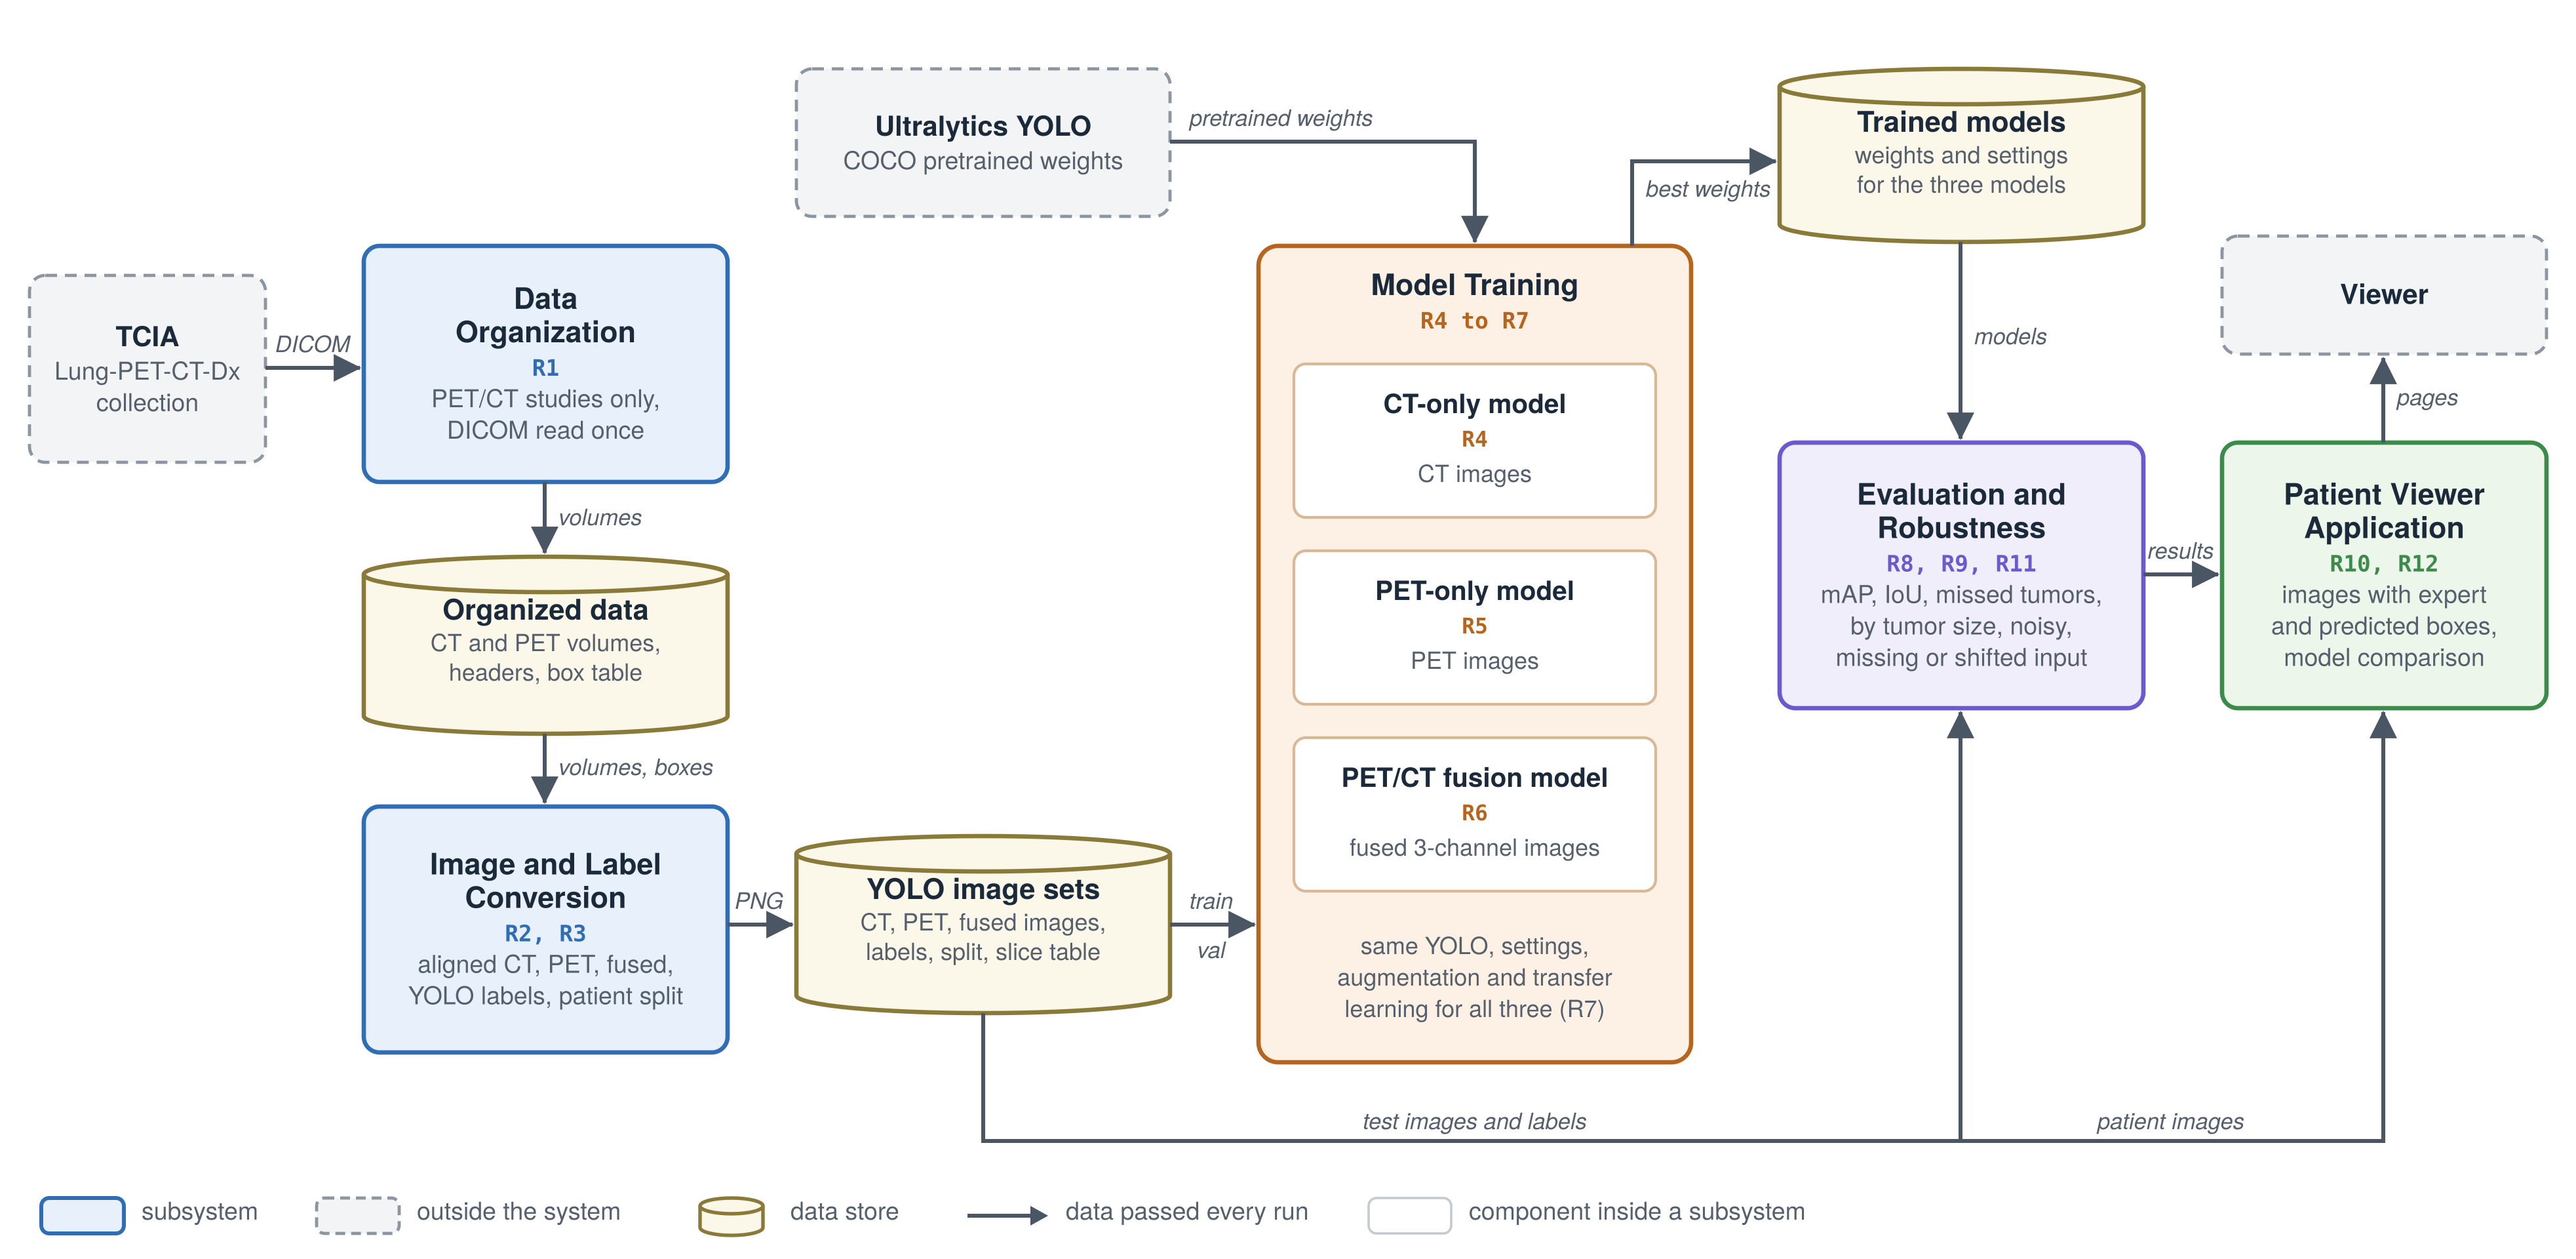
\includegraphics[width=\textwidth]{./figures/SA_P2_LungTumor.png}
	\caption[System architecture of the lung tumor detection system (drawn using Claude).]{\upd{System architecture of the lung tumor detection system (drawn using Claude).}}
	\label{fig:architecture}
\end{figure}

{\color{red}Figure~\ref{fig:architecture} presents the system architecture of ...

\noindent\textbf{Note from Dr.\ Sekmen.} Figure~\ref{fig:architecture} is the reference architecture for this project. Explain it here in your own words, starting with the sentence above. Walk the reader through the figure from left to right. For each subsystem, say what it is responsible for, what it receives, what it produces and which requirements of Chapter~2 it satisfies. Explain the three data stores, the outside sources (TCIA, the pretrained YOLO weights and the viewer) and what each arrow carries. Make clear that DICOM files are read only once, by Data Organization and Image and Label Conversion, and that everything after that works with PNG images and label files. Then add a short traceability table that lists every requirement R1 to R12 against the subsystem that satisfies it. Use the subsystem names of Figure~\ref{fig:architecture} everywhere in this chapter, and delete this red text when you are done.\par}

\upd{Data Organization} is a subsystem in our project that mainly focuses on the dataset we are using, as well as the organization of the dataset. Our project uses the dataset Lung-PET-CT-Dx collection from The Cancer Imaging Archive (TCIA)\upd{. It} contains two different series of scans, CT and PET\upd{. Only patients with a paired PET/CT study are kept, and studies} that do not contain annotations \upd{are excluded}. Each study is then checked for available expert tumor annotations\upd{.} The organized data and tumor annotations are then passed to \upd{Image and Label Conversion} for image preparation and image alignment.

The \upd{Image and Label Conversion} subsystem is responsible for preparing the collected images for tumor detection. Received CT images are processed using lung and mediastinal windows, while PET images are normalized and spatially aligned with the corresponding CT images. The received images are then put into three different input channels, CT-only, PET-only and \upd{PET/CT fusion}. The expert annotations are then converted into YOLO bounding box labels\upd{, and the patients are} split into three different sets, training, validation and testing\upd{, in proportions of} 75/10/15 respectively. The following images and labels are then passed into the next subsystem for model training \upd{and, for the test set, to evaluation. After this step the system no longer reads DICOM files.}

The \upd{Model Training} subsystem is where we apply training and deep learning models to detect tumors in the received images. A pretrained YOLO model is used to train the three independent tumor detection models. All three models will \upd{use} the same pretrained weights, patient data splits and training settings to keep the models on an even playing field for comparison. Once the models are trained and the test images are processed, the models will generate bounding boxes with confidence scores. With those confidence \upd{scores} they are able to be evaluated in the next subsystem\upd{, Evaluation and Robustness,} dealing with the comparison of those scores against each modality, specifically they are measured to compare tumor localization performance of each modality.

The \upd{Evaluation and Robustness} subsystem is responsible for analyzing the tumor detection results produced by the three YOLO models. The subsystem receives \upd{the trained models, runs them on the test images to obtain} predicted tumor bounding boxes and confidence scores\upd{,} and compares them against the expert-provided tumor annotations. The performance of the CT-only, PET-only, and fused PET/CT models is evaluated using metrics such as precision, recall, Intersection over Union (IoU), and mean Average Precision (mAP). Additional analysis examines tumor size, false positives, missed detections, and the effects of noisy, missing, or misaligned imaging data on model performance. \upd{The Patient Viewer Application} provides visual comparisons of the medical images, expert annotations, and predicted tumor locations through a reproducible application. These results allow the performance of the three imaging approaches to be compared and their strengths and limitations to be identified.

\upd{Figures~\ref{fig:team1} and \ref{fig:team2} show the inside of these subsystems in more detail.}

\begin{figure}[htbp]
	\centering
	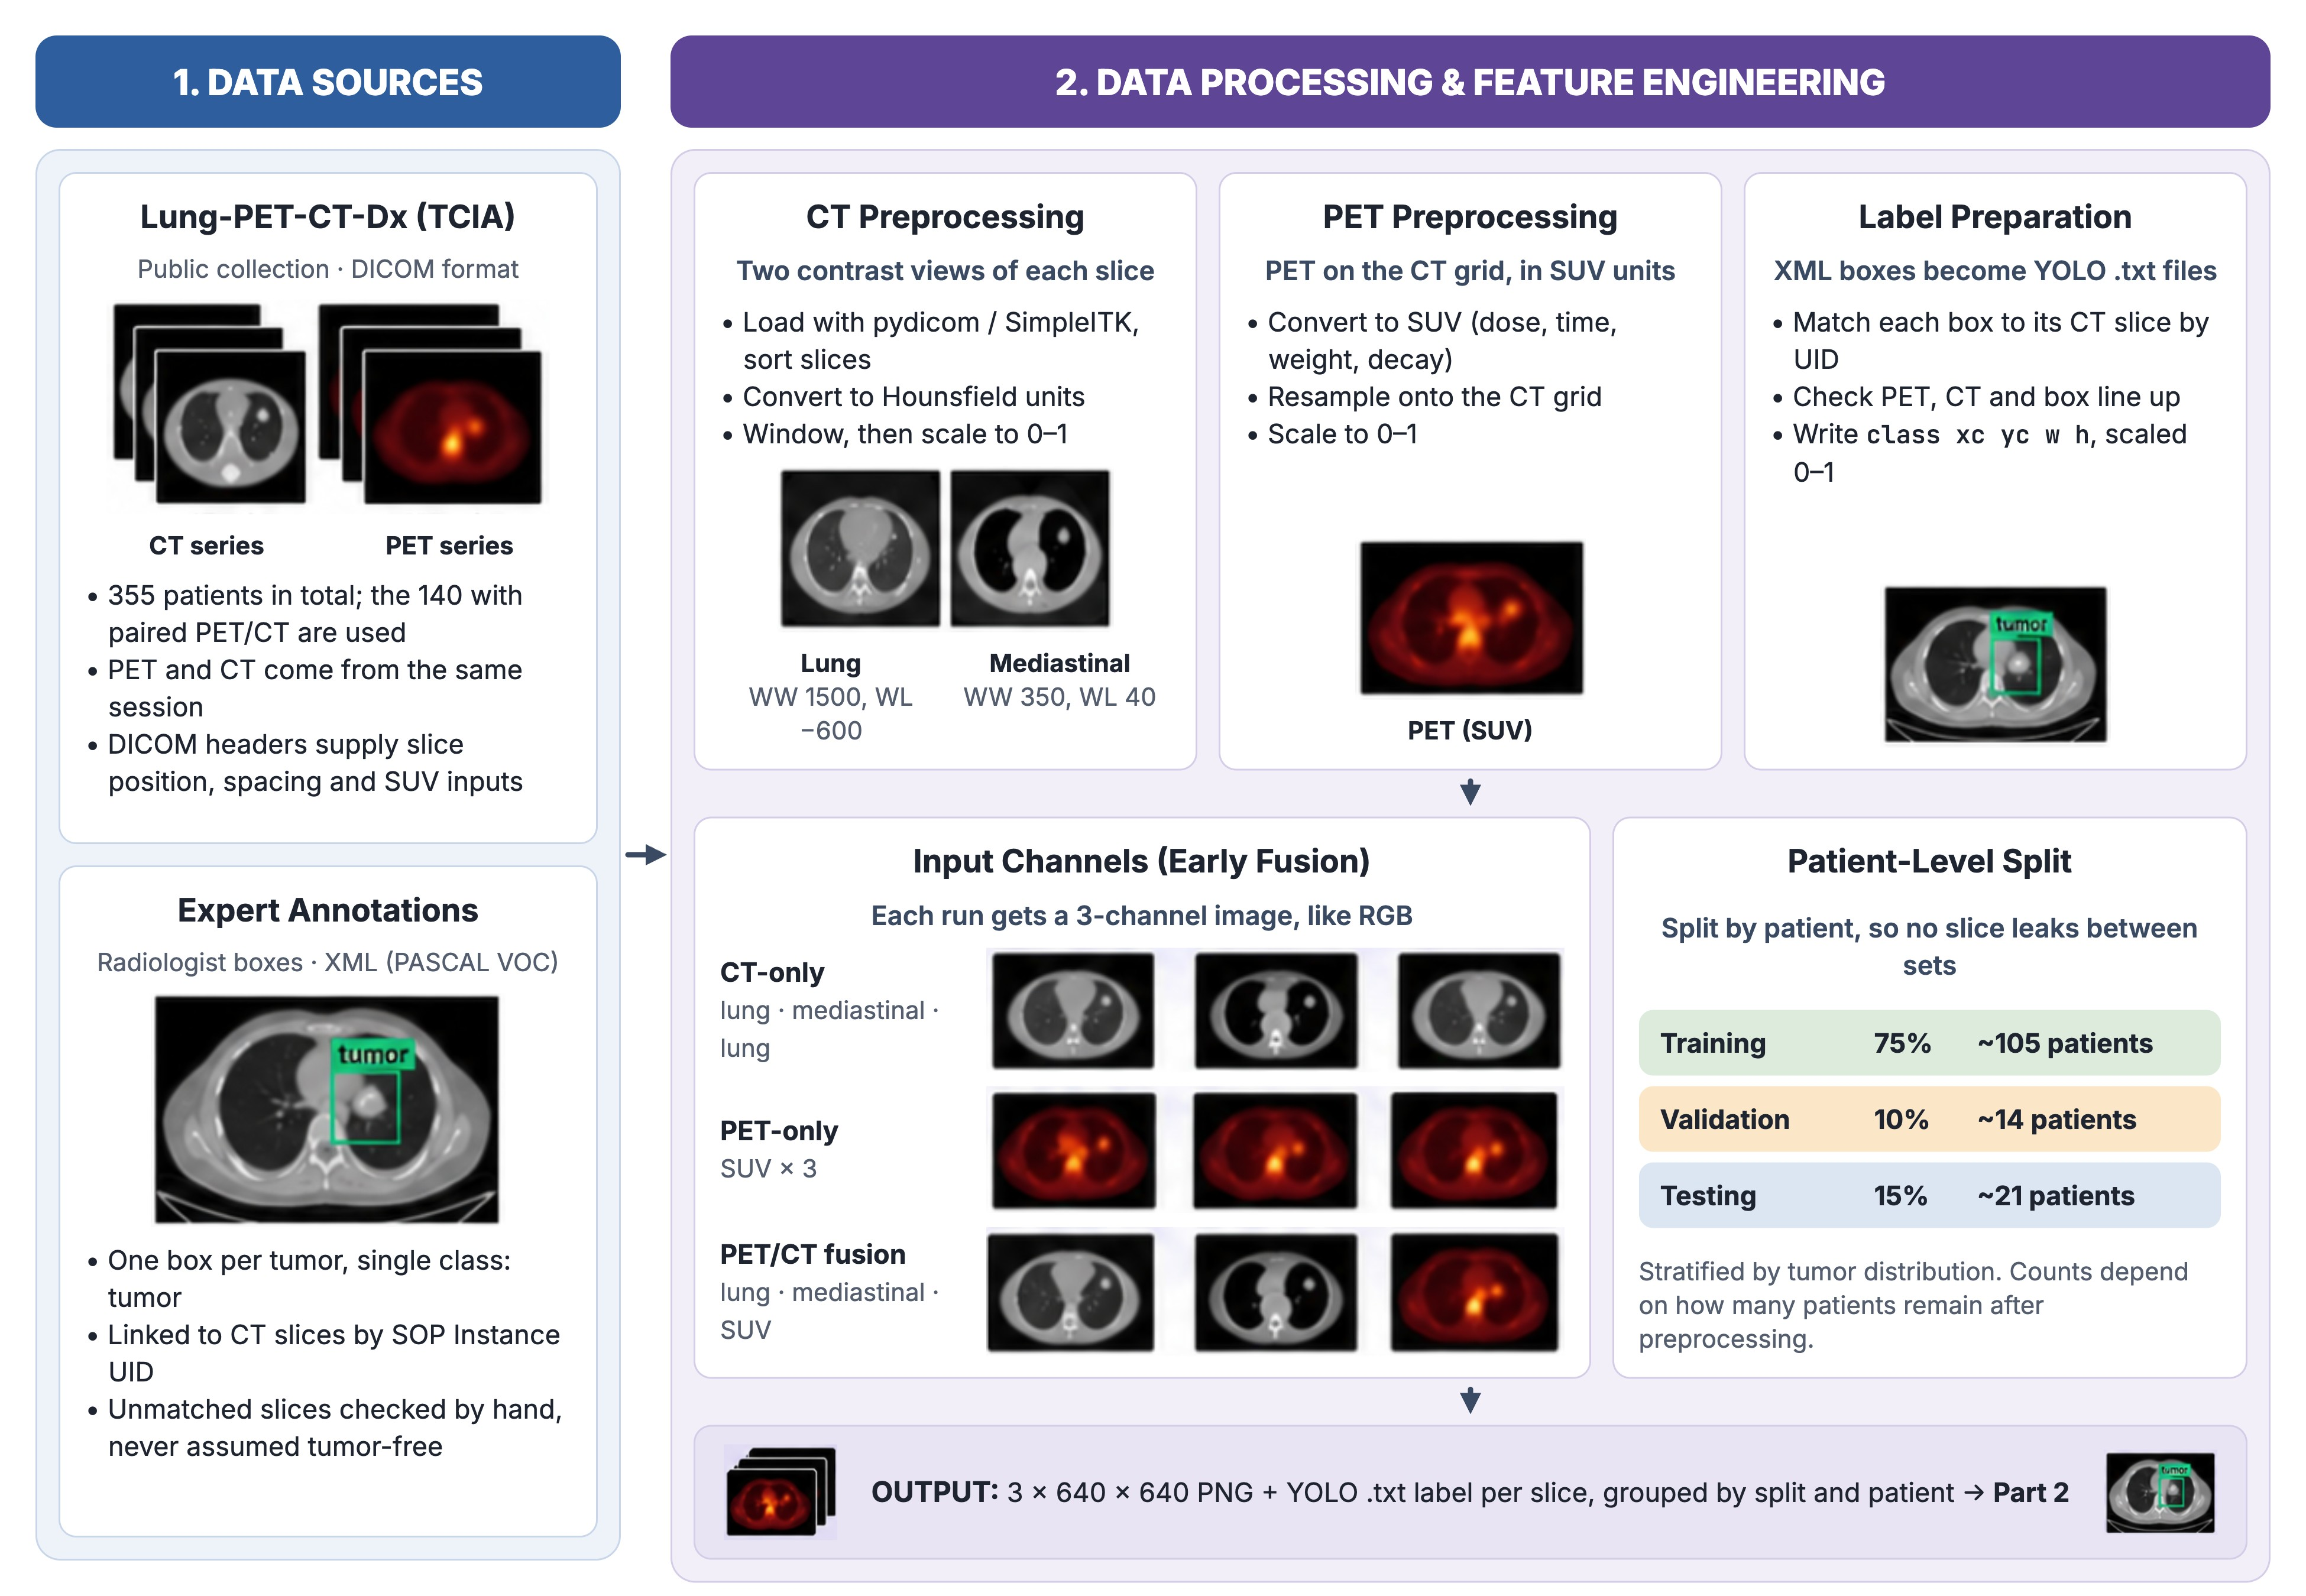
\includegraphics[width=\textwidth]{./figures/Team_DataSources_Processing.jpg}
	\caption[Data Organization and Image and Label Conversion.]{\upd{Data Organization and Image and Label Conversion.}}
	\label{fig:team1}
\end{figure}

\begin{figure}[htbp]
	\centering
	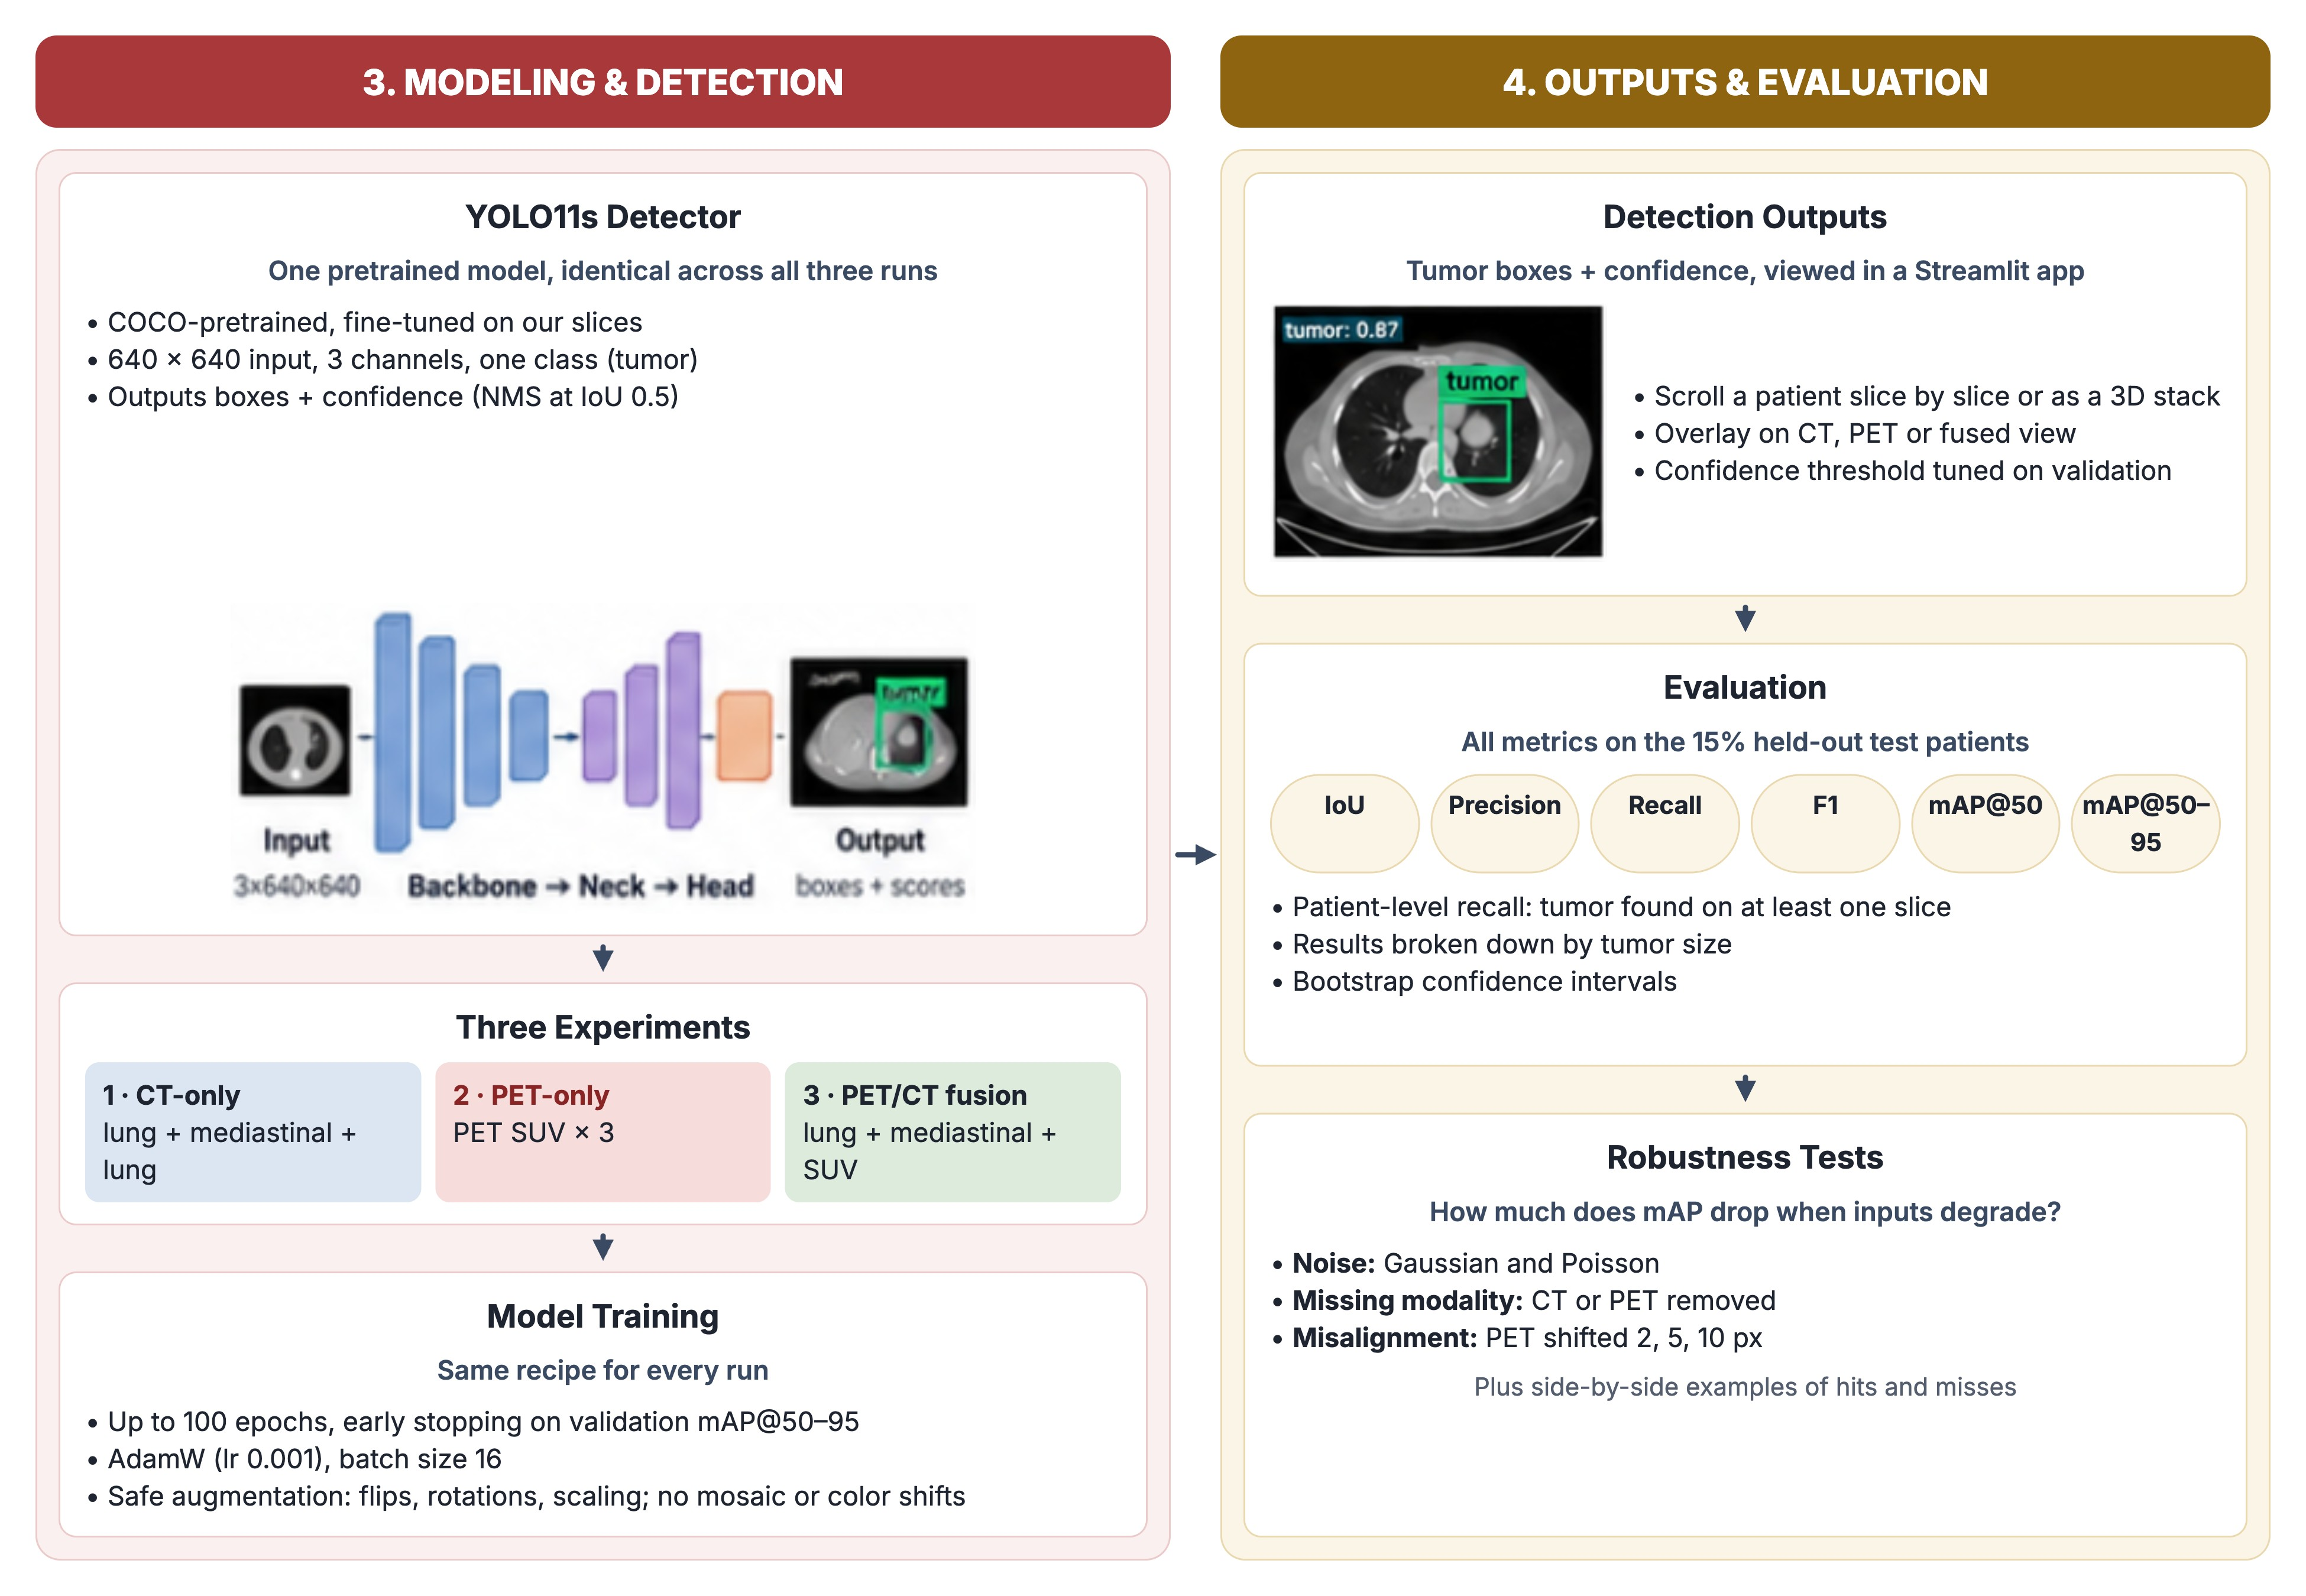
\includegraphics[width=\textwidth]{./figures/Team_Modeling_Outputs.jpg}
	\caption[Model Training, Evaluation and Robustness, and the Patient Viewer Application.]{\upd{Model Training, Evaluation and Robustness, and the Patient Viewer Application.}}
	\label{fig:team2}
\end{figure}

{\color{red}\noindent\textbf{Note from Dr.\ Sekmen.} Retitle the panels of Figures~\ref{fig:team1} and \ref{fig:team2} so they use the subsystem names of Figure~\ref{fig:architecture}. ``Data Sources'' becomes Data Organization, ``Data Processing \& Feature Engineering'' becomes Image and Label Conversion, ``Modeling \& Detection'' becomes Model Training, and ``Outputs \& Evaluation'' becomes Evaluation and Robustness together with the Patient Viewer Application.\par}

% ---------------------------------------------------------------------
\section{Detailed Design}
\label{sec:detailed}
This section explains how each of the \upd{subsystems in Figure~\ref{fig:architecture}} works inside. Each subsystem is divided into components (Figures~\upd{\ref{fig:comp-org} to \ref{fig:comp-eval}}), and the methods, formulas and settings of each component are given here.

% .....................................................................
\subsection[Data Organization]{\upd{Data Organization}}

\begin{figure}[htbp]
	\centering
	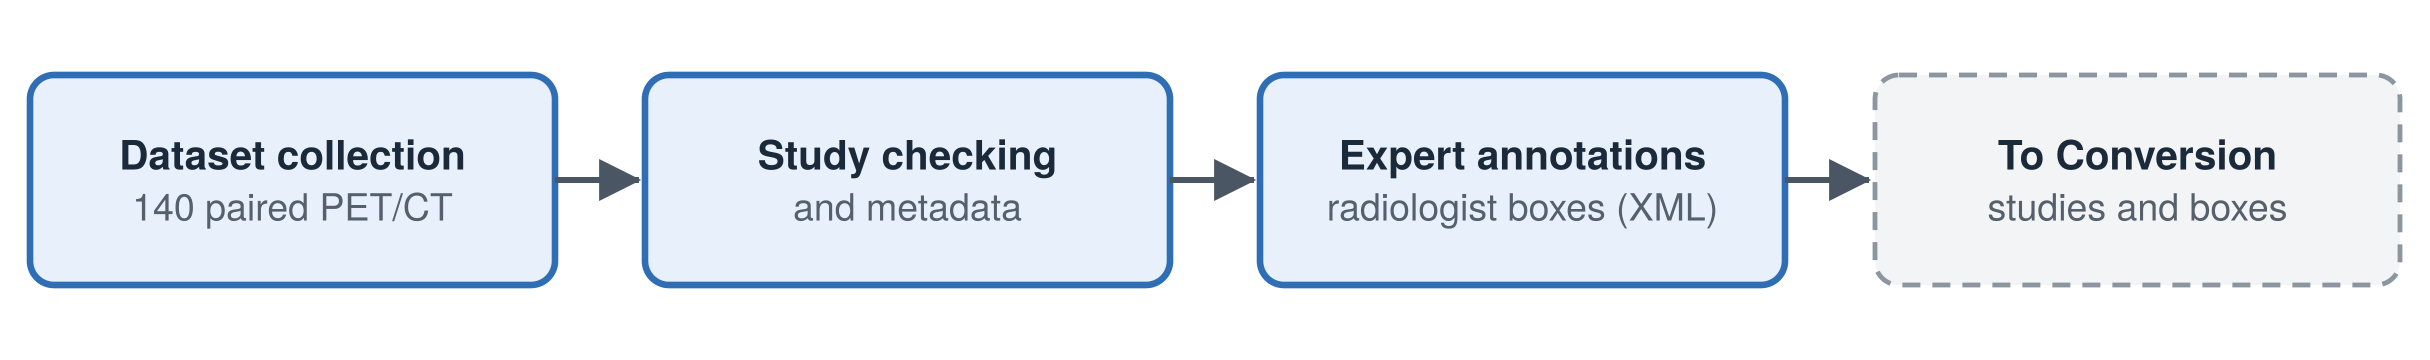
\includegraphics[width=\textwidth]{./figures/Comp_DataOrganization.png}
	\caption[Components of Data Organization.]{Components of \upd{Data Organization}.}
	\label{fig:comp-org}
\end{figure}

\textbf{Dataset collection.} The 140 patients with a paired PET/CT study are taken from the Lung-PET-CT-Dx collection, and the downloaded version is recorded for citation. The series of each patient are organized by patient identifier and passed to study checking.

\textbf{Study checking and metadata.} A study is kept only if its CT, PET and annotations are all present. The DICOM headers supply the slice position and pixel spacing, used for alignment and for tumor size in millimeters, and the dose, injection time, scan time and patient weight, used for the SUV conversion. Studies that cannot be matched reliably are documented and excluded, and the verified CT and PET volumes \upd{are stored in the organized data}.

\textbf{Expert annotations.} Each radiologist box (PASCAL VOC XML) marks one tumor on one CT slice and carries that slice's identifier, which links the box to its image. There is a single class, tumor. The verified boxes are \upd{stored with the volumes and passed to Image and Label Conversion}, where they are converted to YOLO labels.

% .....................................................................
\subsection[Image and Label Conversion]{\upd{Image and Label Conversion}}

\begin{figure}[htbp]
	\centering
	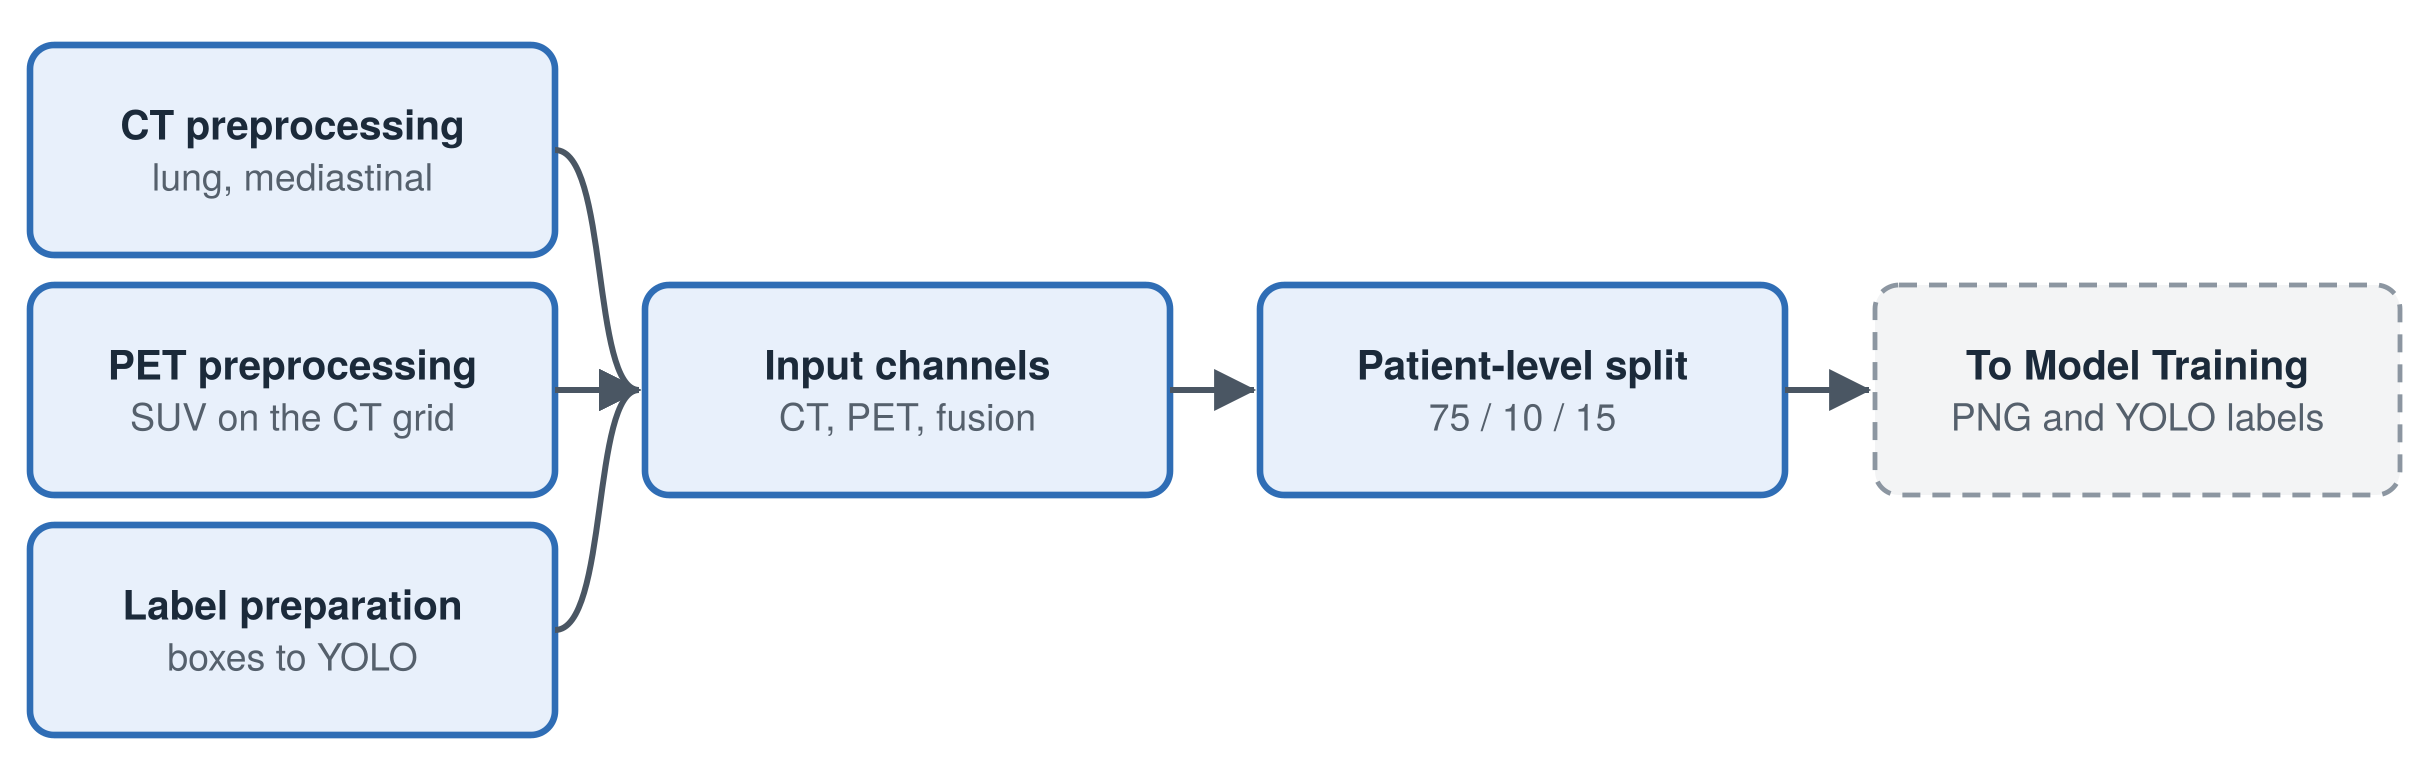
\includegraphics[width=\textwidth]{./figures/Comp_Conversion.png}
	\caption[Components of Image and Label Conversion.]{Components of \upd{Image and Label Conversion}.}
	\label{fig:comp-conv}
\end{figure}

\textbf{CT preprocessing.} CT slices are sorted by position and converted to Hounsfield units (HU). Each slice is windowed twice, with window width $WW$ and level $WL$, and scaled to 0--1:
\begin{equation}
	I = \mathrm{clip}\!\left(\frac{HU - (WL - WW/2)}{WW},\ 0,\ 1\right)
\end{equation}
The lung window ($WW = 1500$, $WL = -600$) covers $-1350$ to $150$ HU; the mediastinal window ($WW = 350$, $WL = 40$) covers $-135$ to $215$ HU. The two windowed images of each slice are passed to input channel construction.

\textbf{PET preprocessing.} Raw PET values are converted to standardized uptake values so they are comparable between patients:
\begin{equation}
	SUV = \frac{C \cdot W}{D_0 \cdot 2^{-\Delta t / T_{1/2}}}
\end{equation}
$C$ is the measured activity concentration, $W$ the patient weight, $D_0$ the injected dose, $\Delta t$ the time from injection to scan, and $T_{1/2}$ the tracer half-life (about 110 minutes for fluorine-18). The volume is then resampled onto the CT grid and scaled to 0--1 with a fixed upper limit of SUV 15. Values above 15 are clipped, so a value of 1 means the same uptake for every patient. The aligned PET images are passed to input channel construction.

\textbf{Label preparation.} Each box is matched to its CT slice by slice identifier (SOP Instance UID), checked against the PET and CT slices, and written as a YOLO line, with image width $W_{img}$ and height $H_{img}$:
\begin{equation}
	x_c = \frac{x_{min} + x_{max}}{2W_{img}}, \quad
	y_c = \frac{y_{min} + y_{max}}{2H_{img}}, \quad
	w = \frac{x_{max} - x_{min}}{W_{img}}, \quad
	h = \frac{y_{max} - y_{min}}{H_{img}}
\end{equation}
The values stay valid when images are resized to $640 \times 640$. Slices with no matching box are checked by hand and never assumed to be tumor-free. The labels stay linked to the CT, PET and fused images of the same slice\upd{, and the patient identifier and pixel spacing of every slice are recorded in a slice table, so later steps never need the DICOM files}.

\textbf{Input channel construction.} Each experiment gets a three-channel image (Table~\ref{tab:channels}). The fusion input stacks the CT lung window, the CT mediastinal window and the aligned PET SUV image, so the channels line up pixel by pixel. Using the same three-channel format for all experiments lets one pretrained detector be used unchanged. The images are saved as $640 \times 640$ PNG files and passed to the patient-level split.

\begin{table}[htbp]
	\centering
	\caption{Channel contents of the three experiments.}
	\label{tab:channels}
	\begin{tabular}{llll}
		\hline
		Experiment & Channel 1 & Channel 2 & Channel 3 \\
		\hline
		CT-only & CT lung window & CT mediastinal window & CT lung window \\
		PET-only & PET SUV & PET SUV & PET SUV \\
		PET/CT fusion & CT lung window & CT mediastinal window & PET SUV \\
		\hline
	\end{tabular}
\end{table}

\textbf{Patient-level split.} Whole patients are assigned to training, validation and testing (about 105, 14 and 21 of 140), stratified by tumor distribution. Splitting by patient keeps near-identical neighboring slices out of different sets, and a check confirms no patient appears in more than one set. The same split is used for all three experiments. The image folders, YOLO label files\upd{, slice table} and dataset configuration files are then \upd{stored in the YOLO image sets}.

% .....................................................................
\subsection[Model Training]{\upd{Model Training}}

\begin{figure}[htbp]
	\centering
	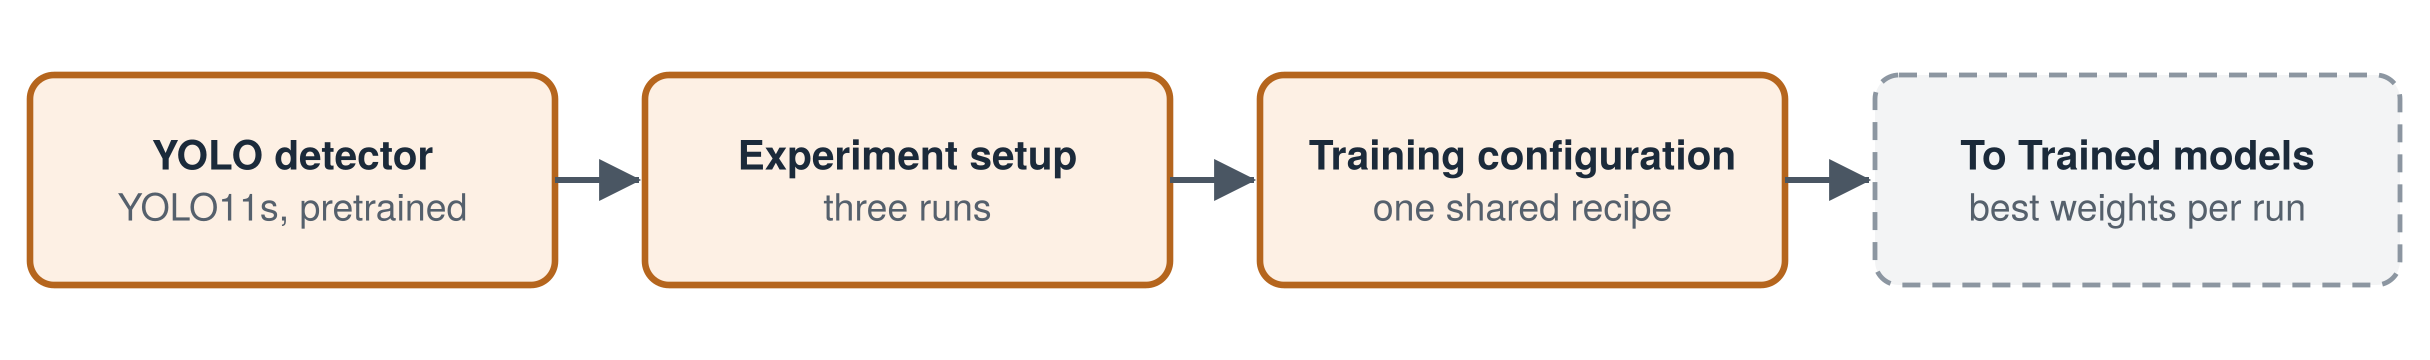
\includegraphics[width=\textwidth]{./figures/Comp_ModelTraining.png}
	\caption[Components of Model Training.]{Components of \upd{Model Training}.}
	\label{fig:comp-train}
\end{figure}

\textbf{YOLO detector.} The detector is YOLO11s, fine-tuned from COCO-pretrained weights. It takes a $640 \times 640$, three-channel image: a backbone extracts features, a neck combines several scales so small and large tumors are both found, and a head predicts boxes and confidence scores for one class, tumor. The same architecture is used for all three experiments.

\textbf{Experiment setup.} The CT-only, PET-only and fusion detectors are trained as three independent runs, each with its own dataset file but with the same starting weights, split and recipe, so only the image content differs. No weights are carried from one experiment to another.

\textbf{Training configuration.} The recipe in Table~\ref{tab:recipe} is applied to every run, and the weights from the best validation epoch are kept. Mosaic and color changes are off because they would mix slices from different patients or mix the CT and PET channels. The configuration and the trained weights are saved separately for each experiment \upd{in the trained models store}.

\begin{table}[htbp]
	\centering
	\caption{Training recipe shared by all three experiments.}
	\label{tab:recipe}
	\begin{tabular}{lp{10cm}}
		\hline
		Input & $640 \times 640$, 3 channels, one class (tumor) \\
		Epochs & Up to 100; early stopping on validation mAP@50--95 (patience 20 epochs) \\
		Optimizer & AdamW, learning rate 0.001, batch size 16 \\
		Augmentation & Flips, rotations, scaling; training images only; no mosaic, no color changes \\
		Random seed & Fixed at 0 and the same for all runs \\
		\hline
	\end{tabular}
\end{table}

% .....................................................................
\subsection[Evaluation and Robustness]{\upd{Evaluation and Robustness}}

\begin{figure}[htbp]
	\centering
	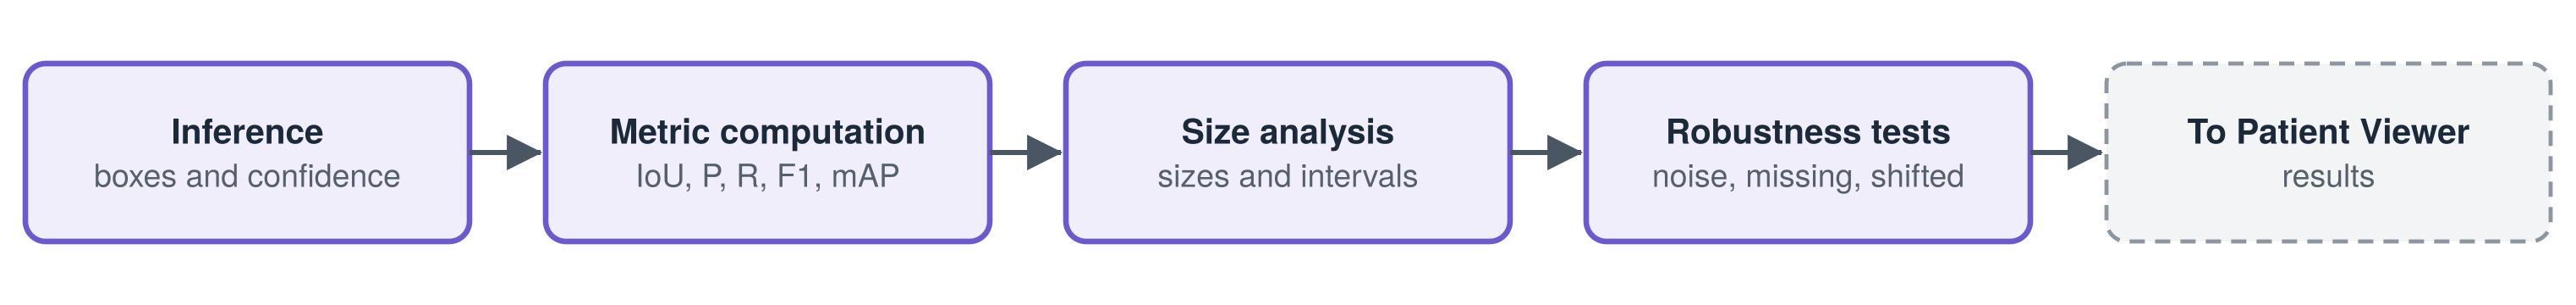
\includegraphics[width=\textwidth]{./figures/Comp_Evaluation.png}
	\caption[Components of Evaluation and Robustness.]{Components of \upd{Evaluation and Robustness}.}
	\label{fig:comp-eval}
\end{figure}

\textbf{Inference.} Each model runs on the test images of its own experiment, and overlapping boxes for the same tumor are merged by non-maximum suppression at an IoU of 0.5. The confidence threshold is chosen on the validation set and then fixed for testing. Each prediction is saved with its patient and slice identifier\upd{.}

\textbf{Metric computation.} A predicted box $P$ is matched to an expert box $E$ by Intersection over Union:
\begin{equation}
	IoU = \frac{\mathrm{area}(P \cap E)}{\mathrm{area}(P \cup E)}
\end{equation}
A match at $IoU \geq 0.5$ (the same value used for non-maximum suppression and for mAP@50) is a true positive ($TP$), an unmatched prediction is a false positive ($FP$), and an unmatched expert box is a false negative ($FN$). The same rule is used for all three models.
\begin{equation}
	\mathrm{Precision} = \frac{TP}{TP + FP}, \quad
	\mathrm{Recall} = \frac{TP}{TP + FN}, \quad
	F_1 = \frac{2 \cdot \mathrm{Precision} \cdot \mathrm{Recall}}{\mathrm{Precision} + \mathrm{Recall}}
\end{equation}
mAP@50 is the mean average precision at IoU 0.5, and mAP@50--95 averages it over IoU 0.50 to 0.95 in steps of 0.05. A patient-level recall counts a tumor as found if at least one of its slices has a matching detection. The results of all three models are saved in one common format so they can be compared directly.

\textbf{Size analysis and intervals.} Tumor size is calculated in millimeters from each expert box and the \upd{pixel spacing in the slice table}, and each tumor is placed in one group by the longer side of its box: small (under 20 mm), medium (20 to 40 mm) or large (over 40 mm). The limits are fixed before the analysis and saved with the evaluation settings. Because only about 21 patients are tested, the test patients are resampled with replacement 1,000 times, every metric is recomputed, and the middle 95\% of values is reported as the interval. The component also compares the saved predictions case by case, to find tumors that one model detects and another misses, and to list the false positives and missed tumors of each model, including cases where the fused model differs from CT-only or PET-only.

\textbf{Robustness tests.} Degradations are applied to copies of the test images and the trained models are not retrained. Gaussian and Poisson noise are applied to all three models. For the fusion model, either the CT channels or the PET channel is removed, and the PET channel is shifted by 2, 5 or 10 pixels. The drop is measured against the clean result:
\begin{equation}
	\Delta mAP = mAP_{clean} - mAP_{degraded}
\end{equation}
The results are saved for each model and test condition, which shows how sensitive the three approaches are to noise, missing information and misalignment.

% .....................................................................
\subsection[Patient Viewer Application]{\upd{Patient Viewer Application}}

\textbf{Detection viewer.} A Streamlit application lets a reviewer pick a test patient, scroll the slices or step through the 3D stack, and view predicted boxes with confidence scores on the CT, PET or fused view. It only reads saved images and predictions, so it shows exactly what was evaluated. The final results, representative images and robustness comparisons are available through the \upd{same} application.
). Figures are in ./figures/.
% Black text is the team's original text.
% Blue text is an update by Dr. Sekmen.
% Red text is a note from Dr. Sekmen and must be removed when addressed.
% =====================================================================
\providecommand{\upd}[1]{\textcolor{blue}{#1}}

\chapter{Design}
{\color{blue}This chapter explains how the system meets the functional requirements of Chapter~2. Section~\ref{sec:architecture} presents the architectural design. It shows the major subsystems, the data stores between them, the data that moves from one subsystem to another, and the outside sources the system depends on. Section~\ref{sec:detailed} presents the detailed design. Each subsystem is divided into components, and the methods, formulas and settings of each component are given.\par}

% ---------------------------------------------------------------------
\section[Architectural Design]{\upd{Architectural Design}}
\label{sec:architecture}

\begin{figure}[htbp]
	\centering
	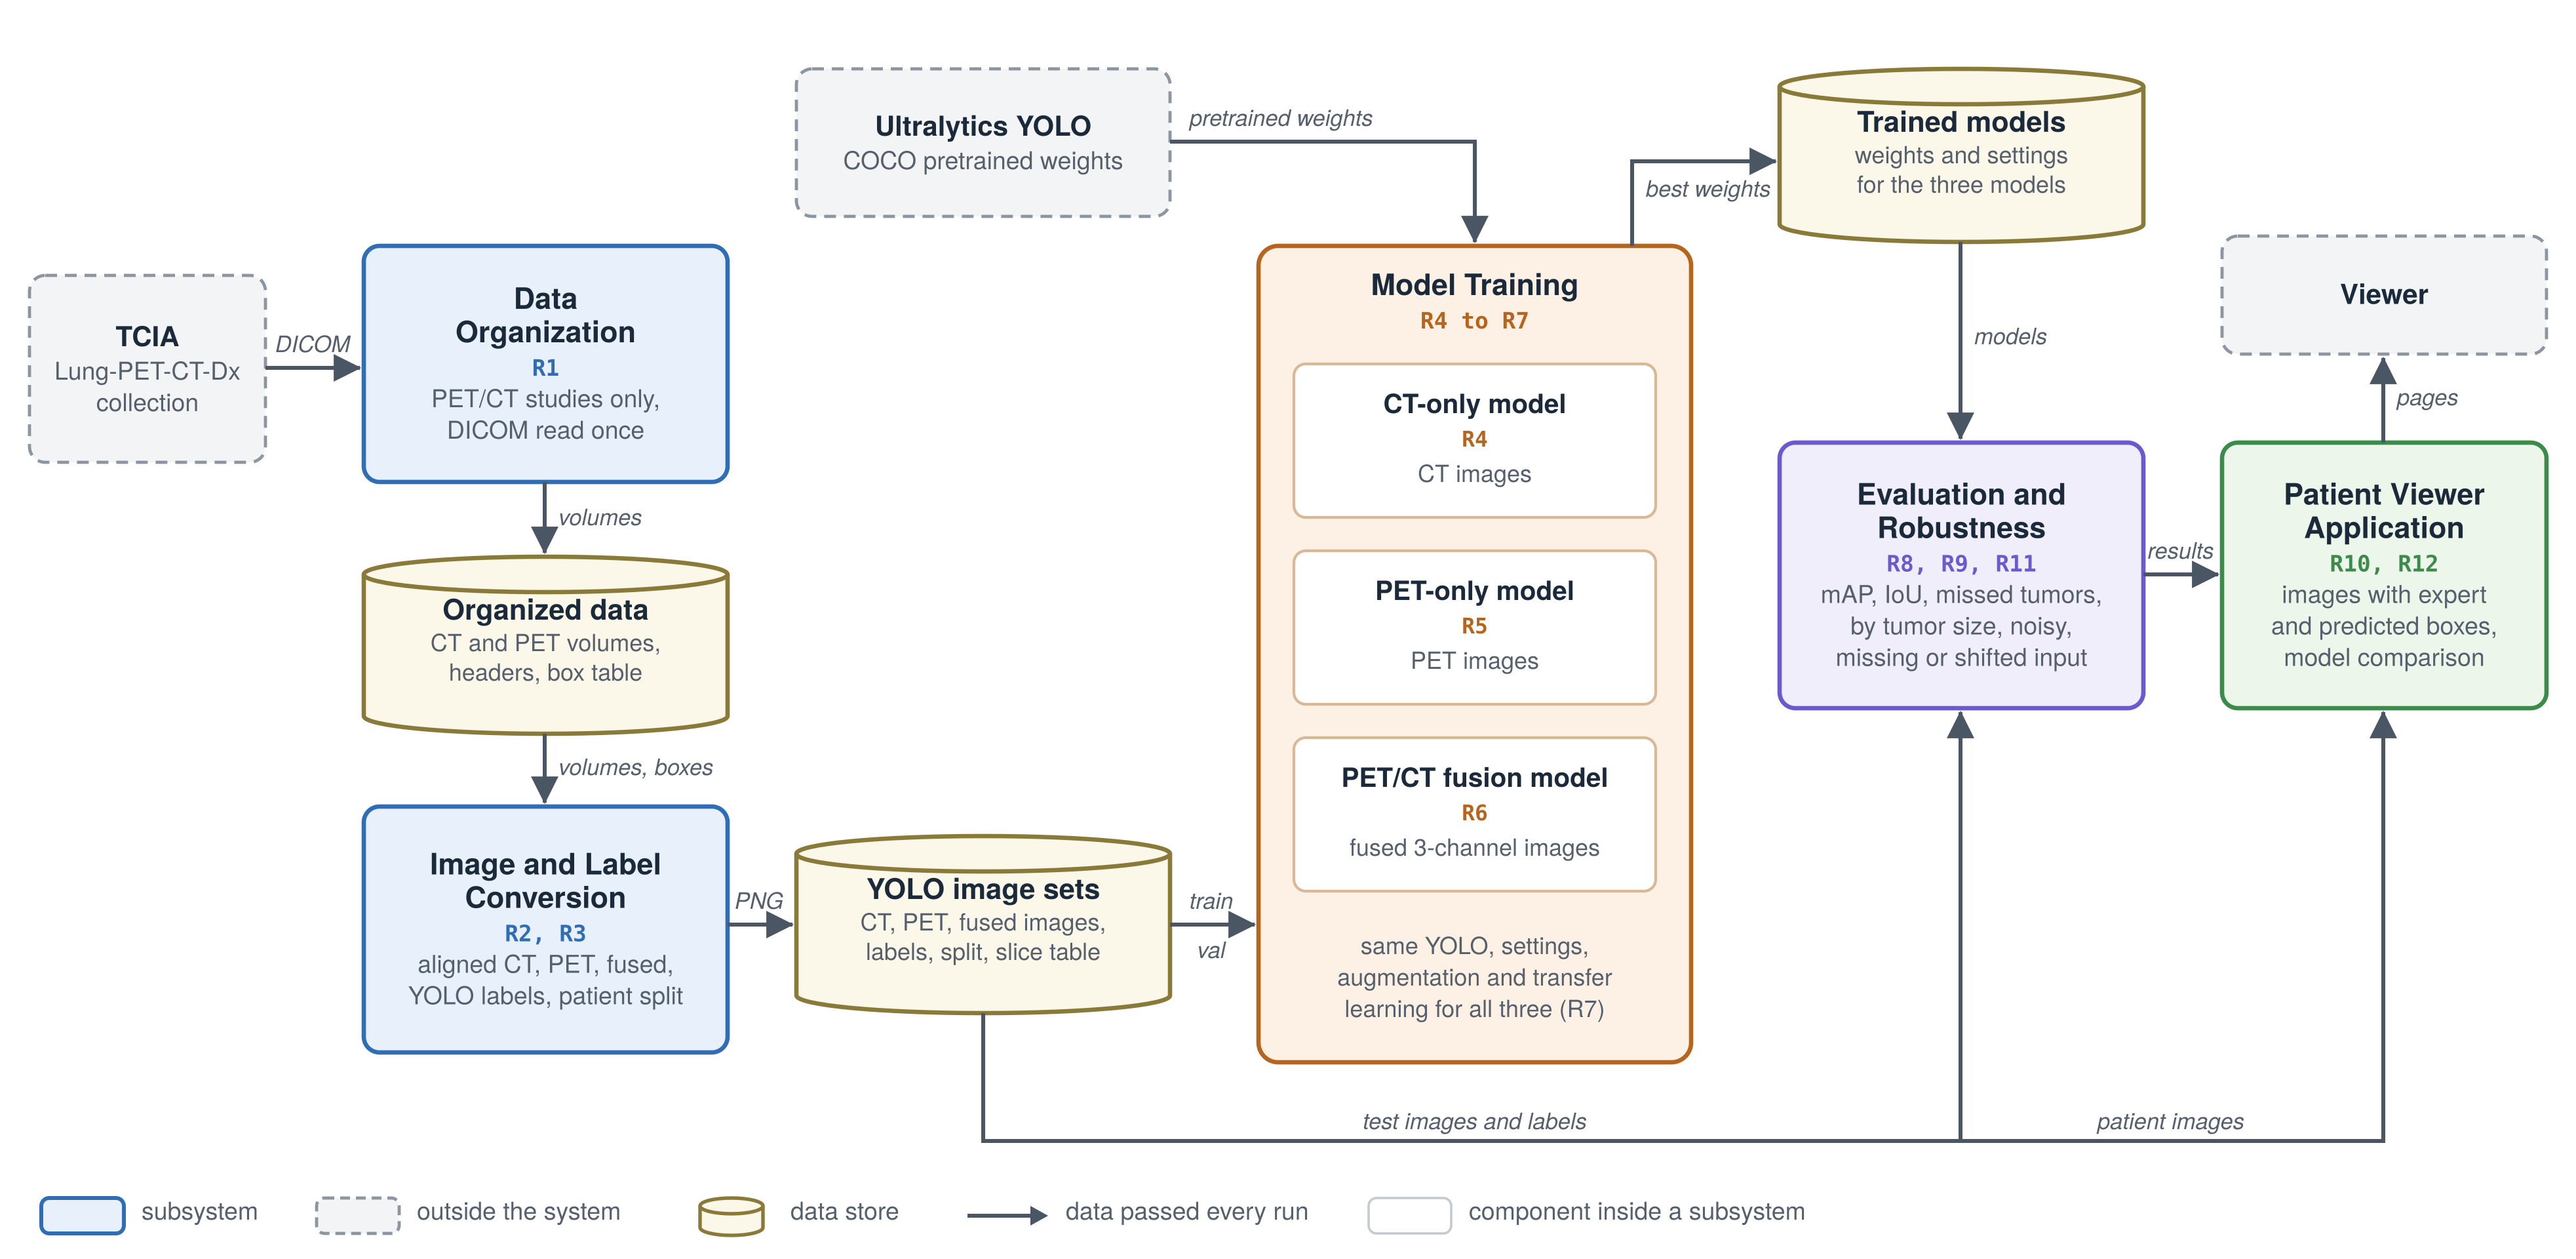
\includegraphics[width=\textwidth]{./figures/SA_P2_LungTumor.png}
	\caption[System architecture of the lung tumor detection system (drawn using Claude).]{\upd{System architecture of the lung tumor detection system (drawn using Claude).}}
	\label{fig:architecture}
\end{figure}

{\color{red}Figure~\ref{fig:architecture} presents the system architecture of ...

\noindent\textbf{Note from Dr.\ Sekmen.} Figure~\ref{fig:architecture} is the reference architecture for this project. Explain it here in your own words, starting with the sentence above. Walk the reader through the figure from left to right. For each subsystem, say what it is responsible for, what it receives, what it produces and which requirements of Chapter~2 it satisfies. Explain the three data stores, the outside sources (TCIA, the pretrained YOLO weights and the viewer) and what each arrow carries. Make clear that DICOM files are read only once, by Data Organization and Image and Label Conversion, and that everything after that works with PNG images and label files. Then add a short traceability table that lists every requirement R1 to R12 against the subsystem that satisfies it. Use the subsystem names of Figure~\ref{fig:architecture} everywhere in this chapter, and delete this red text when you are done.\par}

\upd{Data Organization} is a subsystem in our project that mainly focuses on the dataset we are using, as well as the organization of the dataset. Our project uses the dataset Lung-PET-CT-Dx collection from The Cancer Imaging Archive (TCIA)\upd{. It} contains two different series of scans, CT and PET\upd{. Only patients with a paired PET/CT study are kept, and studies} that do not contain annotations \upd{are excluded}. Each study is then checked for available expert tumor annotations\upd{.} The organized data and tumor annotations are then passed to \upd{Image and Label Conversion} for image preparation and image alignment.

The \upd{Image and Label Conversion} subsystem is responsible for preparing the collected images for tumor detection. Received CT images are processed using lung and mediastinal windows, while PET images are normalized and spatially aligned with the corresponding CT images. The received images are then put into three different input channels, CT-only, PET-only and \upd{PET/CT fusion}. The expert annotations are then converted into YOLO bounding box labels\upd{, and the patients are} split into three different sets, training, validation and testing\upd{, in proportions of} 75/10/15 respectively. The following images and labels are then passed into the next subsystem for model training \upd{and, for the test set, to evaluation. After this step the system no longer reads DICOM files.}

The \upd{Model Training} subsystem is where we apply training and deep learning models to detect tumors in the received images. A pretrained YOLO model is used to train the three independent tumor detection models. All three models will \upd{use} the same pretrained weights, patient data splits and training settings to keep the models on an even playing field for comparison. Once the models are trained and the test images are processed, the models will generate bounding boxes with confidence scores. With those confidence \upd{scores} they are able to be evaluated in the next subsystem\upd{, Evaluation and Robustness,} dealing with the comparison of those scores against each modality, specifically they are measured to compare tumor localization performance of each modality.

The \upd{Evaluation and Robustness} subsystem is responsible for analyzing the tumor detection results produced by the three YOLO models. The subsystem receives \upd{the trained models, runs them on the test images to obtain} predicted tumor bounding boxes and confidence scores\upd{,} and compares them against the expert-provided tumor annotations. The performance of the CT-only, PET-only, and fused PET/CT models is evaluated using metrics such as precision, recall, Intersection over Union (IoU), and mean Average Precision (mAP). Additional analysis examines tumor size, false positives, missed detections, and the effects of noisy, missing, or misaligned imaging data on model performance. \upd{The Patient Viewer Application} provides visual comparisons of the medical images, expert annotations, and predicted tumor locations through a reproducible application. These results allow the performance of the three imaging approaches to be compared and their strengths and limitations to be identified.

\upd{Figures~\ref{fig:team1} and \ref{fig:team2} show the inside of these subsystems in more detail.}

\begin{figure}[htbp]
	\centering
	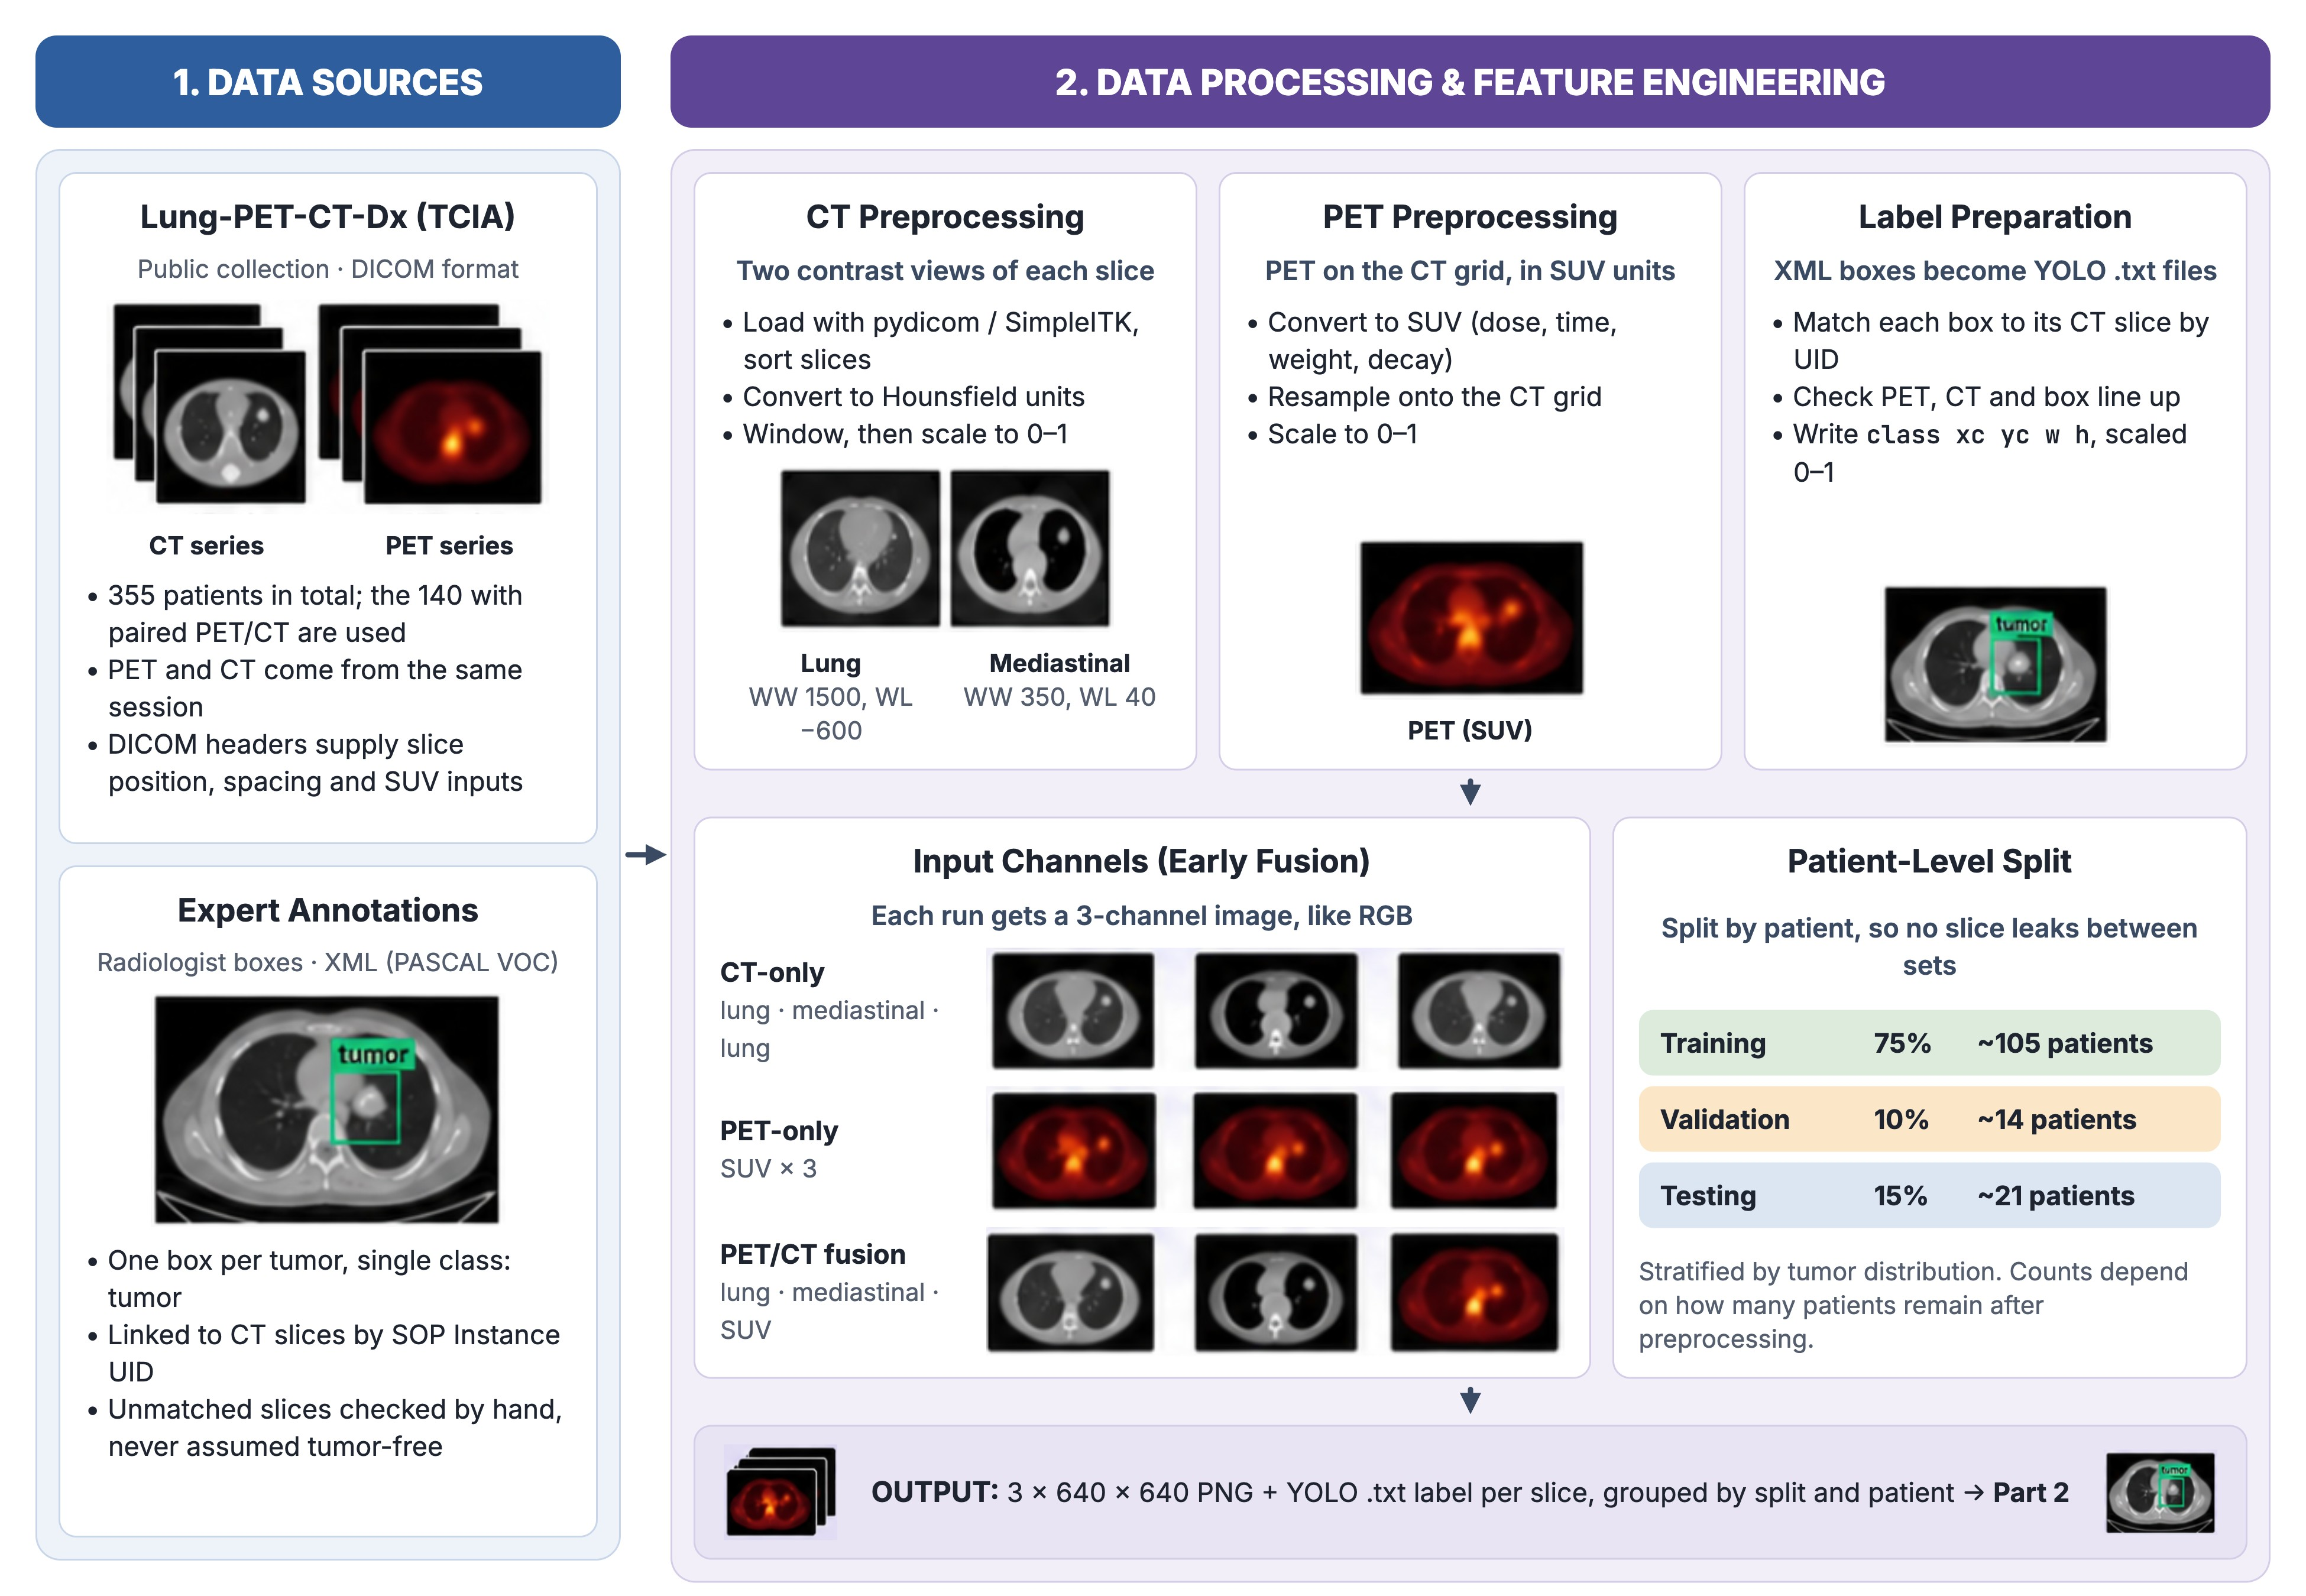
\includegraphics[width=\textwidth]{./figures/Team_DataSources_Processing.jpg}
	\caption[Data Organization and Image and Label Conversion.]{\upd{Data Organization and Image and Label Conversion.}}
	\label{fig:team1}
\end{figure}

\begin{figure}[htbp]
	\centering
	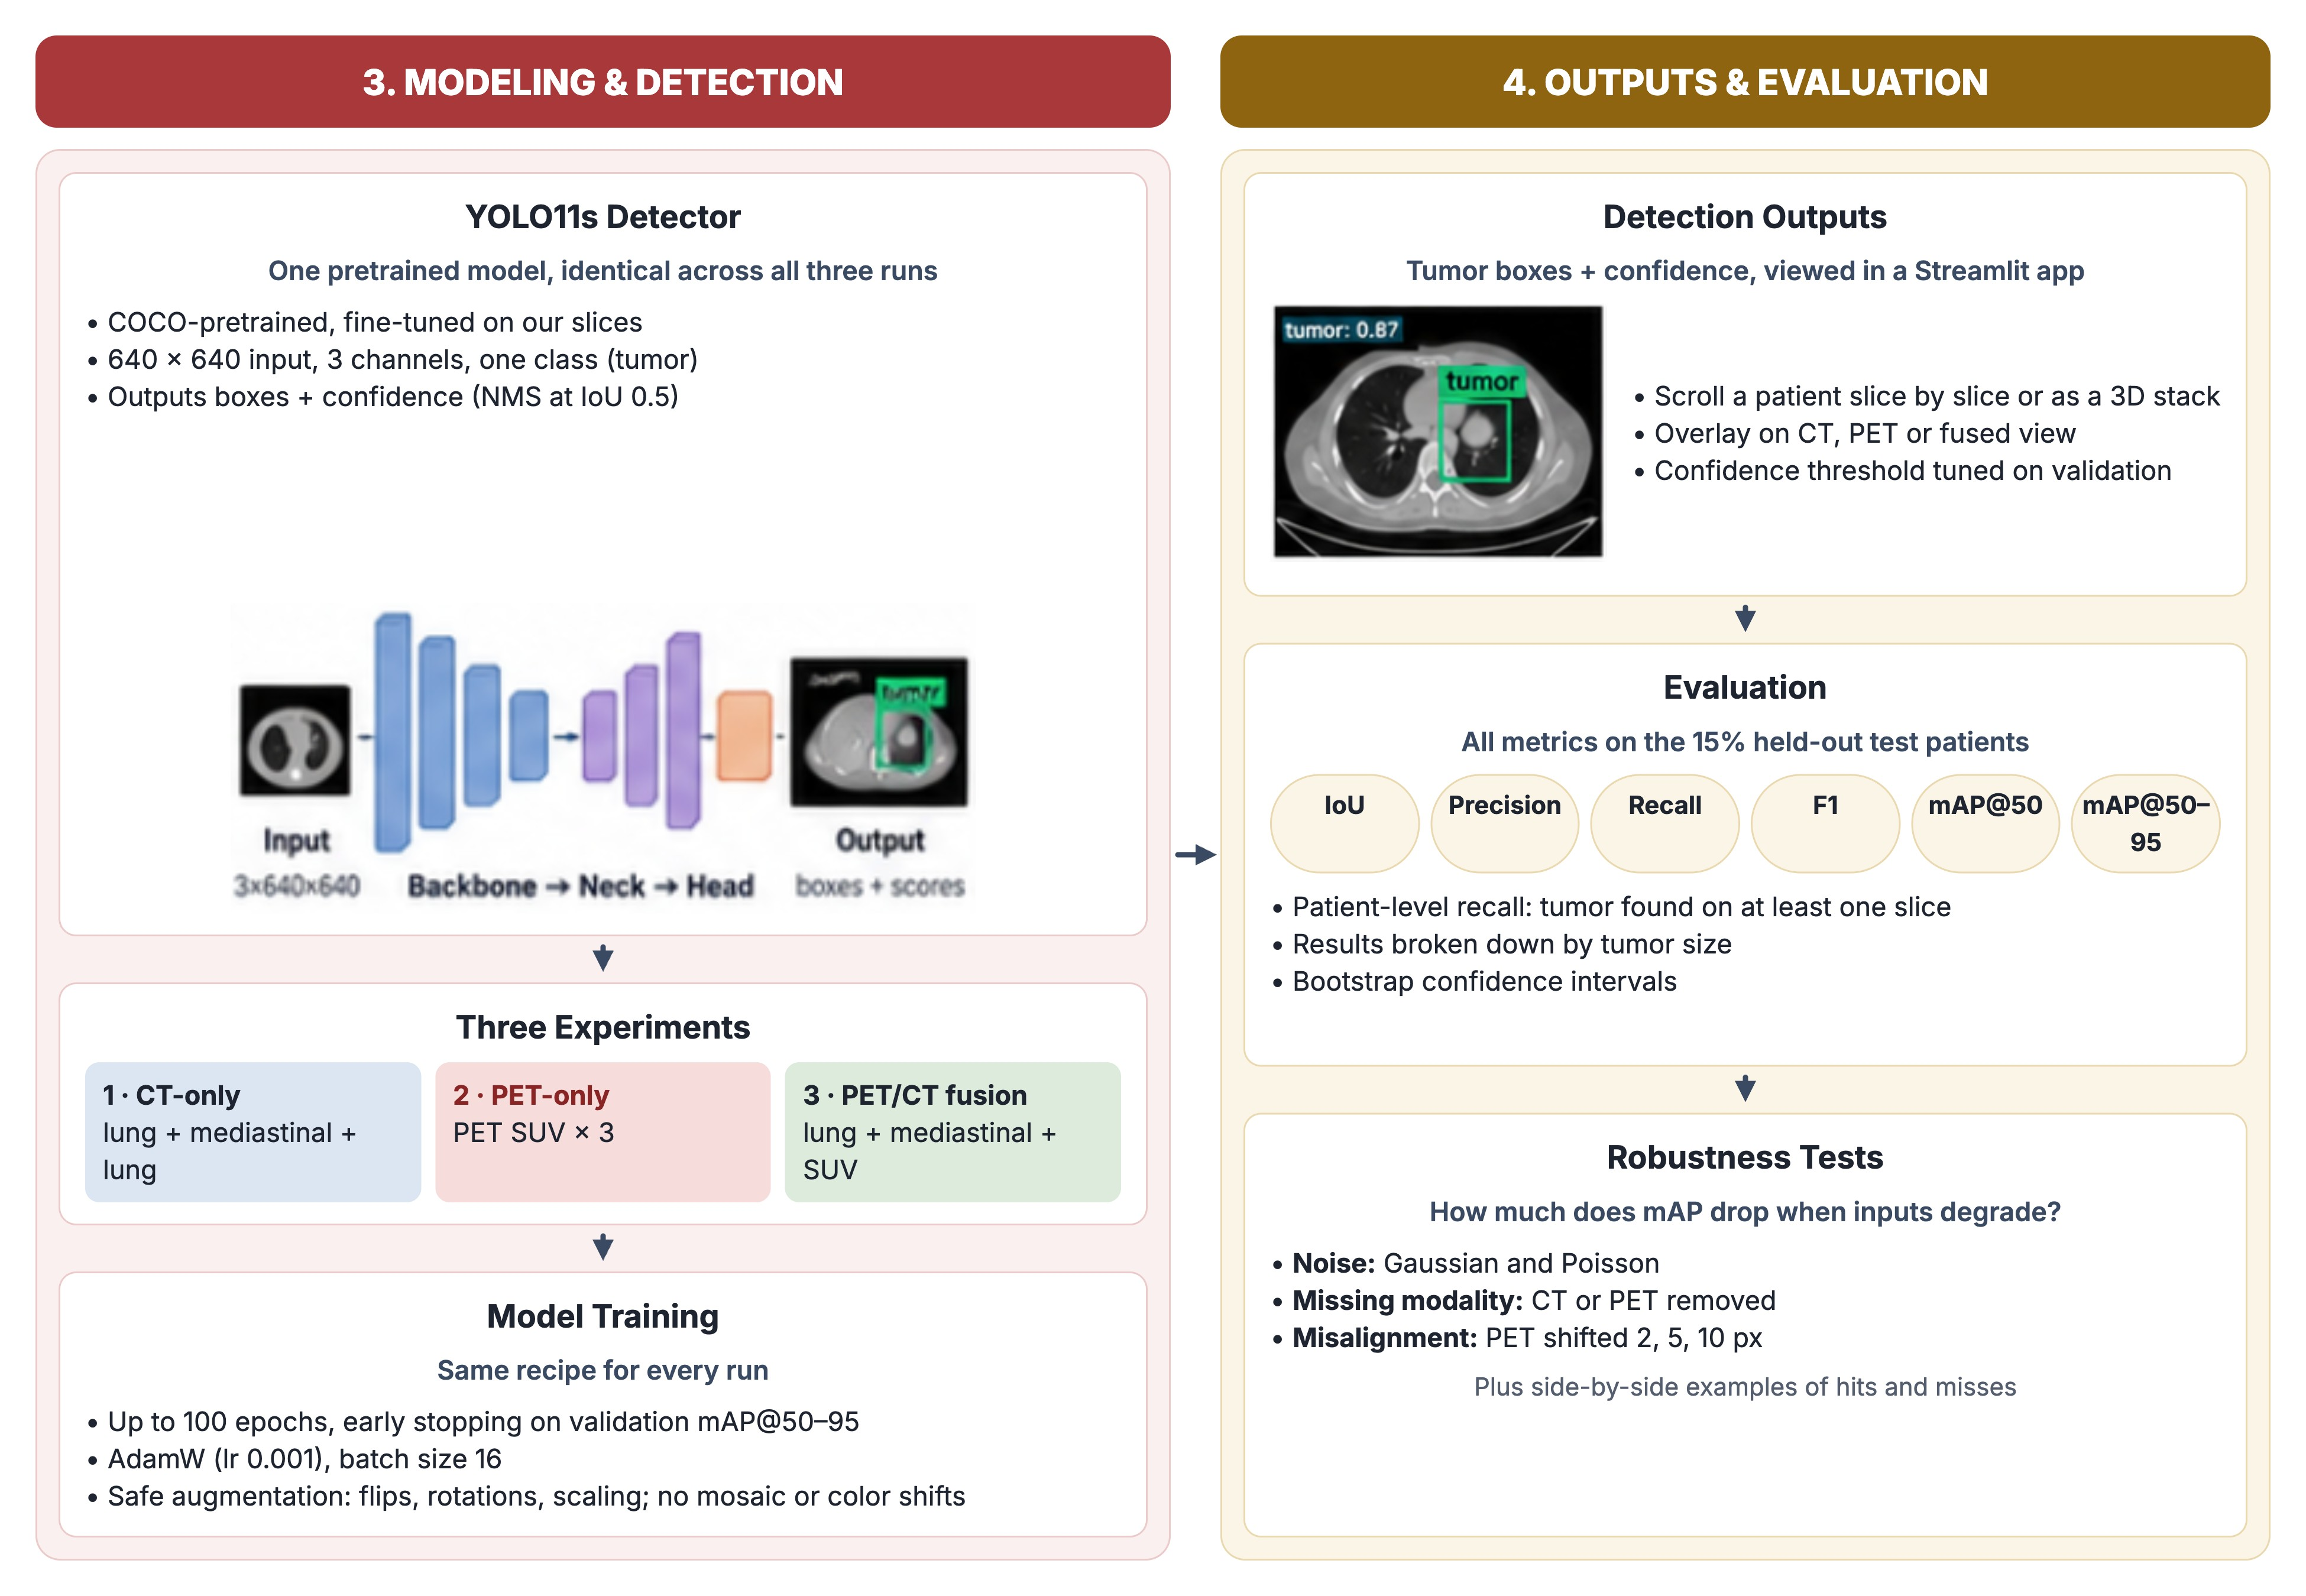
\includegraphics[width=\textwidth]{./figures/Team_Modeling_Outputs.jpg}
	\caption[Model Training, Evaluation and Robustness, and the Patient Viewer Application.]{\upd{Model Training, Evaluation and Robustness, and the Patient Viewer Application.}}
	\label{fig:team2}
\end{figure}

{\color{red}\noindent\textbf{Note from Dr.\ Sekmen.} Retitle the panels of Figures~\ref{fig:team1} and \ref{fig:team2} so they use the subsystem names of Figure~\ref{fig:architecture}. ``Data Sources'' becomes Data Organization, ``Data Processing \& Feature Engineering'' becomes Image and Label Conversion, ``Modeling \& Detection'' becomes Model Training, and ``Outputs \& Evaluation'' becomes Evaluation and Robustness together with the Patient Viewer Application.\par}

% ---------------------------------------------------------------------
\section{Detailed Design}
\label{sec:detailed}
This section explains how each of the \upd{subsystems in Figure~\ref{fig:architecture}} works inside. Each subsystem is divided into components (Figures~\upd{\ref{fig:comp-org} to \ref{fig:comp-eval}}), and the methods, formulas and settings of each component are given here.

% .....................................................................
\subsection[Data Organization]{\upd{Data Organization}}

\begin{figure}[htbp]
	\centering
	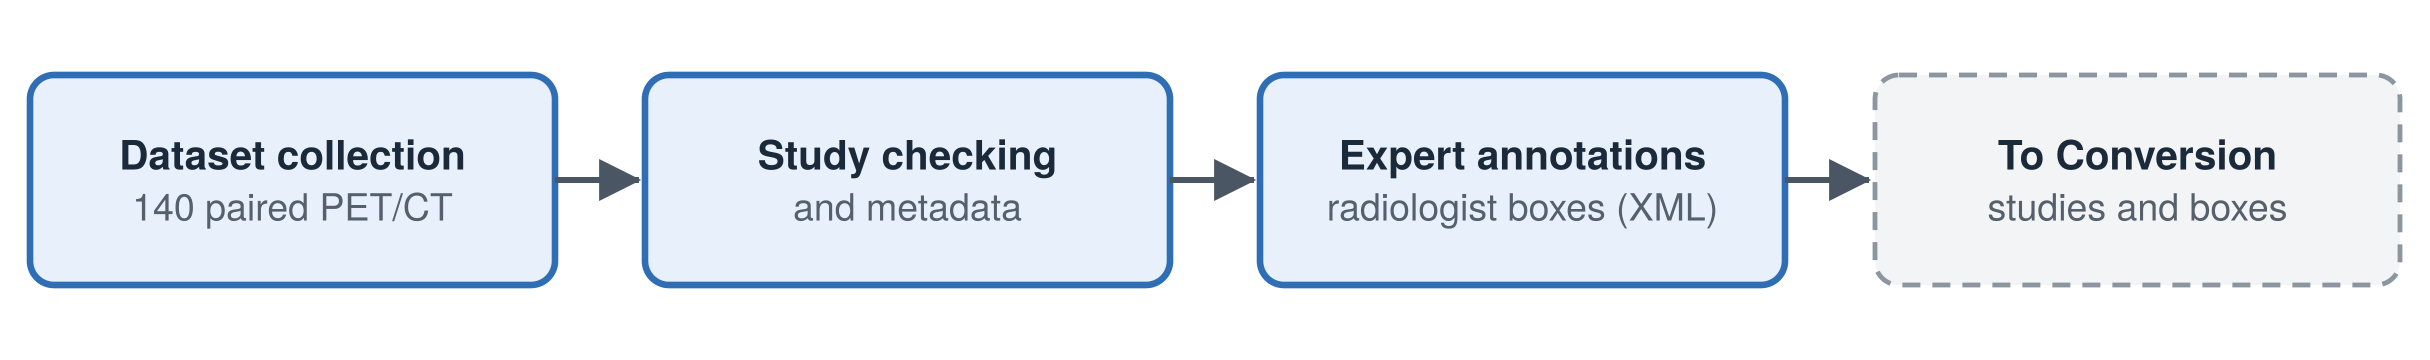
\includegraphics[width=\textwidth]{./figures/Comp_DataOrganization.png}
	\caption[Components of Data Organization.]{Components of \upd{Data Organization}.}
	\label{fig:comp-org}
\end{figure}

\textbf{Dataset collection.} The 140 patients with a paired PET/CT study are taken from the Lung-PET-CT-Dx collection, and the downloaded version is recorded for citation. The series of each patient are organized by patient identifier and passed to study checking.

\textbf{Study checking and metadata.} A study is kept only if its CT, PET and annotations are all present. The DICOM headers supply the slice position and pixel spacing, used for alignment and for tumor size in millimeters, and the dose, injection time, scan time and patient weight, used for the SUV conversion. Studies that cannot be matched reliably are documented and excluded, and the verified CT and PET volumes \upd{are stored in the organized data}.

\textbf{Expert annotations.} Each radiologist box (PASCAL VOC XML) marks one tumor on one CT slice and carries that slice's identifier, which links the box to its image. There is a single class, tumor. The verified boxes are \upd{stored with the volumes and passed to Image and Label Conversion}, where they are converted to YOLO labels.

% .....................................................................
\subsection[Image and Label Conversion]{\upd{Image and Label Conversion}}

\begin{figure}[htbp]
	\centering
	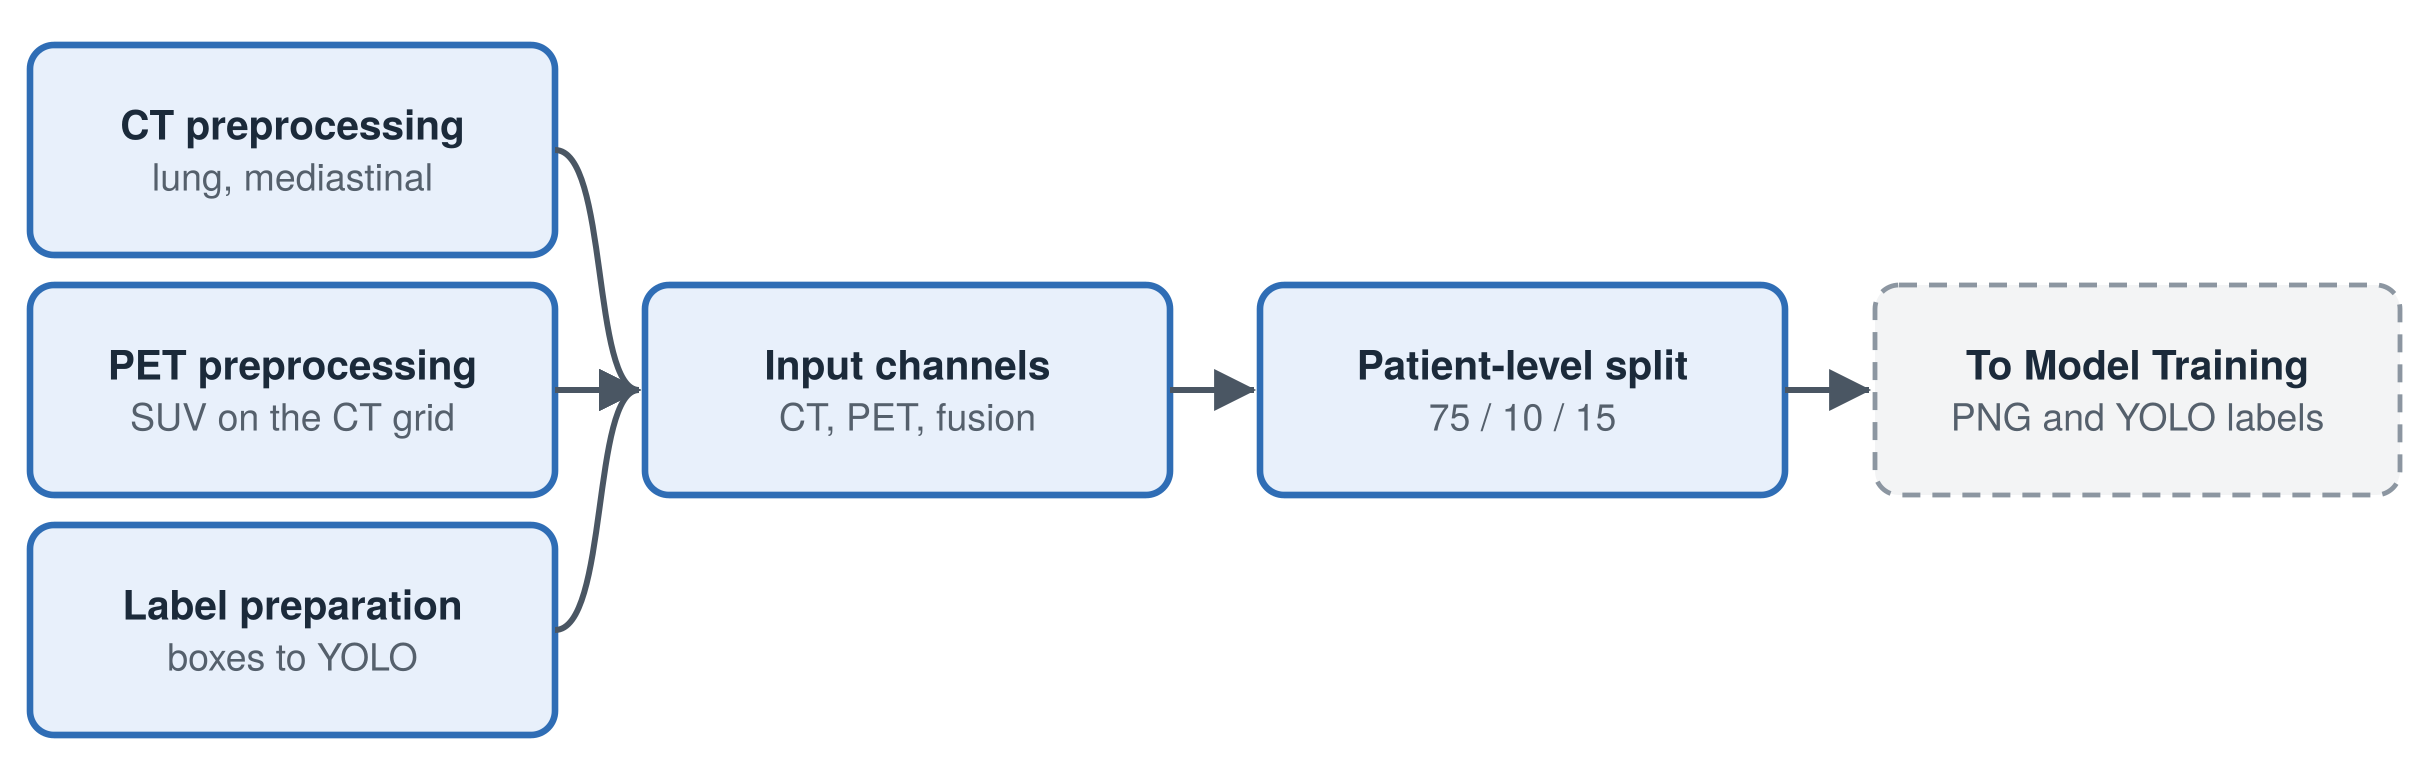
\includegraphics[width=\textwidth]{./figures/Comp_Conversion.png}
	\caption[Components of Image and Label Conversion.]{Components of \upd{Image and Label Conversion}.}
	\label{fig:comp-conv}
\end{figure}

\textbf{CT preprocessing.} CT slices are sorted by position and converted to Hounsfield units (HU). Each slice is windowed twice, with window width $WW$ and level $WL$, and scaled to 0--1:
\begin{equation}
	I = \mathrm{clip}\!\left(\frac{HU - (WL - WW/2)}{WW},\ 0,\ 1\right)
\end{equation}
The lung window ($WW = 1500$, $WL = -600$) covers $-1350$ to $150$ HU; the mediastinal window ($WW = 350$, $WL = 40$) covers $-135$ to $215$ HU. The two windowed images of each slice are passed to input channel construction.

\textbf{PET preprocessing.} Raw PET values are converted to standardized uptake values so they are comparable between patients:
\begin{equation}
	SUV = \frac{C \cdot W}{D_0 \cdot 2^{-\Delta t / T_{1/2}}}
\end{equation}
$C$ is the measured activity concentration, $W$ the patient weight, $D_0$ the injected dose, $\Delta t$ the time from injection to scan, and $T_{1/2}$ the tracer half-life (about 110 minutes for fluorine-18). The volume is then resampled onto the CT grid and scaled to 0--1 with a fixed upper limit of SUV 15. Values above 15 are clipped, so a value of 1 means the same uptake for every patient. The aligned PET images are passed to input channel construction.

\textbf{Label preparation.} Each box is matched to its CT slice by slice identifier (SOP Instance UID), checked against the PET and CT slices, and written as a YOLO line, with image width $W_{img}$ and height $H_{img}$:
\begin{equation}
	x_c = \frac{x_{min} + x_{max}}{2W_{img}}, \quad
	y_c = \frac{y_{min} + y_{max}}{2H_{img}}, \quad
	w = \frac{x_{max} - x_{min}}{W_{img}}, \quad
	h = \frac{y_{max} - y_{min}}{H_{img}}
\end{equation}
The values stay valid when images are resized to $640 \times 640$. Slices with no matching box are checked by hand and never assumed to be tumor-free. The labels stay linked to the CT, PET and fused images of the same slice\upd{, and the patient identifier and pixel spacing of every slice are recorded in a slice table, so later steps never need the DICOM files}.

\textbf{Input channel construction.} Each experiment gets a three-channel image (Table~\ref{tab:channels}). The fusion input stacks the CT lung window, the CT mediastinal window and the aligned PET SUV image, so the channels line up pixel by pixel. Using the same three-channel format for all experiments lets one pretrained detector be used unchanged. The images are saved as $640 \times 640$ PNG files and passed to the patient-level split.

\begin{table}[htbp]
	\centering
	\caption{Channel contents of the three experiments.}
	\label{tab:channels}
	\begin{tabular}{llll}
		\hline
		Experiment & Channel 1 & Channel 2 & Channel 3 \\
		\hline
		CT-only & CT lung window & CT mediastinal window & CT lung window \\
		PET-only & PET SUV & PET SUV & PET SUV \\
		PET/CT fusion & CT lung window & CT mediastinal window & PET SUV \\
		\hline
	\end{tabular}
\end{table}

\textbf{Patient-level split.} Whole patients are assigned to training, validation and testing (about 105, 14 and 21 of 140), stratified by tumor distribution. Splitting by patient keeps near-identical neighboring slices out of different sets, and a check confirms no patient appears in more than one set. The same split is used for all three experiments. The image folders, YOLO label files\upd{, slice table} and dataset configuration files are then \upd{stored in the YOLO image sets}.

% .....................................................................
\subsection[Model Training]{\upd{Model Training}}

\begin{figure}[htbp]
	\centering
	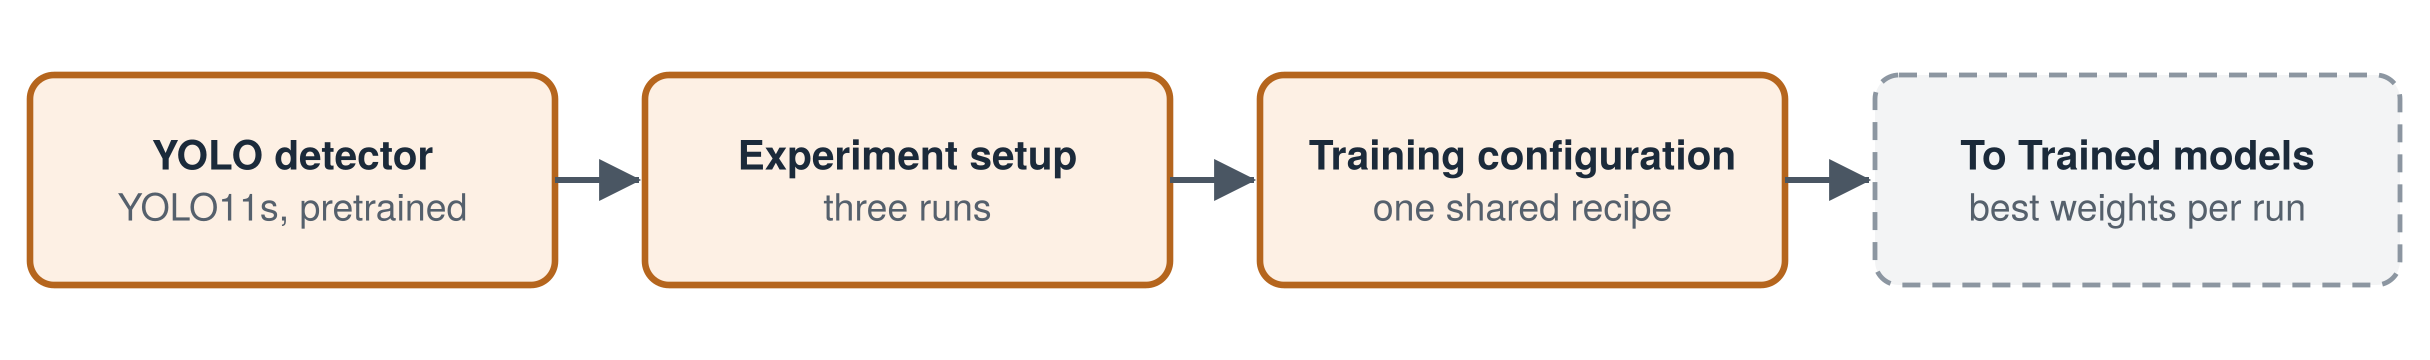
\includegraphics[width=\textwidth]{./figures/Comp_ModelTraining.png}
	\caption[Components of Model Training.]{Components of \upd{Model Training}.}
	\label{fig:comp-train}
\end{figure}

\textbf{YOLO detector.} The detector is YOLO11s, fine-tuned from COCO-pretrained weights. It takes a $640 \times 640$, three-channel image: a backbone extracts features, a neck combines several scales so small and large tumors are both found, and a head predicts boxes and confidence scores for one class, tumor. The same architecture is used for all three experiments.

\textbf{Experiment setup.} The CT-only, PET-only and fusion detectors are trained as three independent runs, each with its own dataset file but with the same starting weights, split and recipe, so only the image content differs. No weights are carried from one experiment to another.

\textbf{Training configuration.} The recipe in Table~\ref{tab:recipe} is applied to every run, and the weights from the best validation epoch are kept. Mosaic and color changes are off because they would mix slices from different patients or mix the CT and PET channels. The configuration and the trained weights are saved separately for each experiment \upd{in the trained models store}.

\begin{table}[htbp]
	\centering
	\caption{Training recipe shared by all three experiments.}
	\label{tab:recipe}
	\begin{tabular}{lp{10cm}}
		\hline
		Input & $640 \times 640$, 3 channels, one class (tumor) \\
		Epochs & Up to 100; early stopping on validation mAP@50--95 (patience 20 epochs) \\
		Optimizer & AdamW, learning rate 0.001, batch size 16 \\
		Augmentation & Flips, rotations, scaling; training images only; no mosaic, no color changes \\
		Random seed & Fixed at 0 and the same for all runs \\
		\hline
	\end{tabular}
\end{table}

% .....................................................................
\subsection[Evaluation and Robustness]{\upd{Evaluation and Robustness}}

\begin{figure}[htbp]
	\centering
	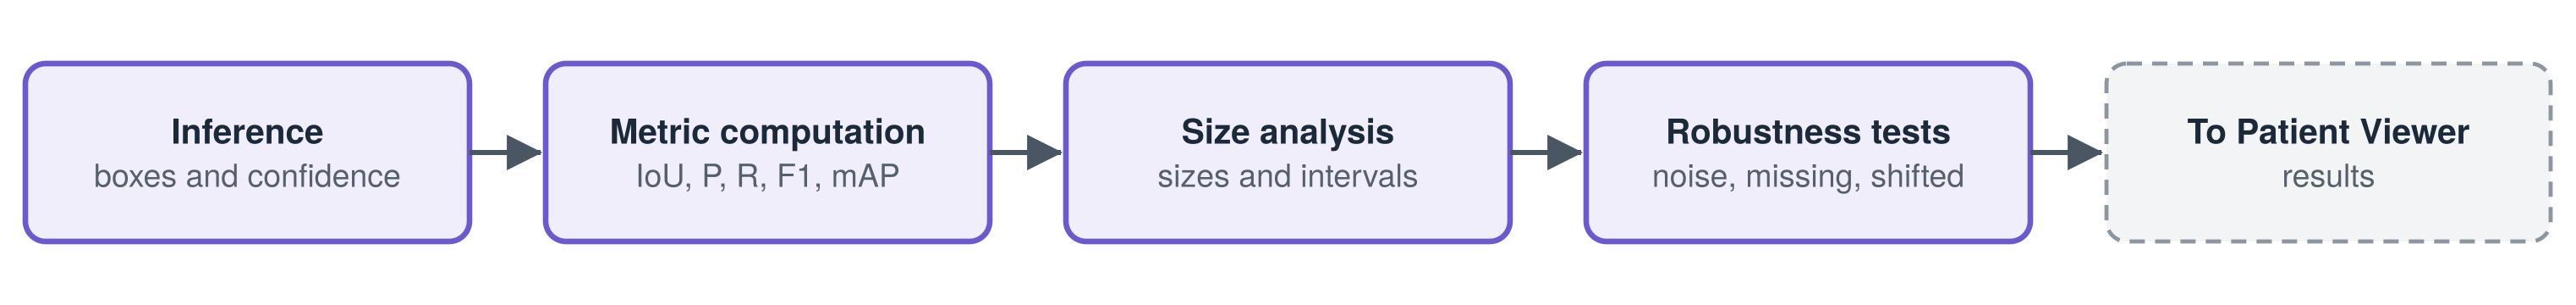
\includegraphics[width=\textwidth]{./figures/Comp_Evaluation.png}
	\caption[Components of Evaluation and Robustness.]{Components of \upd{Evaluation and Robustness}.}
	\label{fig:comp-eval}
\end{figure}

\textbf{Inference.} Each model runs on the test images of its own experiment, and overlapping boxes for the same tumor are merged by non-maximum suppression at an IoU of 0.5. The confidence threshold is chosen on the validation set and then fixed for testing. Each prediction is saved with its patient and slice identifier\upd{.}

\textbf{Metric computation.} A predicted box $P$ is matched to an expert box $E$ by Intersection over Union:
\begin{equation}
	IoU = \frac{\mathrm{area}(P \cap E)}{\mathrm{area}(P \cup E)}
\end{equation}
A match at $IoU \geq 0.5$ (the same value used for non-maximum suppression and for mAP@50) is a true positive ($TP$), an unmatched prediction is a false positive ($FP$), and an unmatched expert box is a false negative ($FN$). The same rule is used for all three models.
\begin{equation}
	\mathrm{Precision} = \frac{TP}{TP + FP}, \quad
	\mathrm{Recall} = \frac{TP}{TP + FN}, \quad
	F_1 = \frac{2 \cdot \mathrm{Precision} \cdot \mathrm{Recall}}{\mathrm{Precision} + \mathrm{Recall}}
\end{equation}
mAP@50 is the mean average precision at IoU 0.5, and mAP@50--95 averages it over IoU 0.50 to 0.95 in steps of 0.05. A patient-level recall counts a tumor as found if at least one of its slices has a matching detection. The results of all three models are saved in one common format so they can be compared directly.

\textbf{Size analysis and intervals.} Tumor size is calculated in millimeters from each expert box and the \upd{pixel spacing in the slice table}, and each tumor is placed in one group by the longer side of its box: small (under 20 mm), medium (20 to 40 mm) or large (over 40 mm). The limits are fixed before the analysis and saved with the evaluation settings. Because only about 21 patients are tested, the test patients are resampled with replacement 1,000 times, every metric is recomputed, and the middle 95\% of values is reported as the interval. The component also compares the saved predictions case by case, to find tumors that one model detects and another misses, and to list the false positives and missed tumors of each model, including cases where the fused model differs from CT-only or PET-only.

\textbf{Robustness tests.} Degradations are applied to copies of the test images and the trained models are not retrained. Gaussian and Poisson noise are applied to all three models. For the fusion model, either the CT channels or the PET channel is removed, and the PET channel is shifted by 2, 5 or 10 pixels. The drop is measured against the clean result:
\begin{equation}
	\Delta mAP = mAP_{clean} - mAP_{degraded}
\end{equation}
The results are saved for each model and test condition, which shows how sensitive the three approaches are to noise, missing information and misalignment.

% .....................................................................
\subsection[Patient Viewer Application]{\upd{Patient Viewer Application}}

\textbf{Detection viewer.} A Streamlit application lets a reviewer pick a test patient, scroll the slices or step through the 3D stack, and view predicted boxes with confidence scores on the CT, PET or fused view. It only reads saved images and predictions, so it shows exactly what was evaluated. The final results, representative images and robustness comparisons are available through the \upd{same} application.
). Figures are in ./figures/.
% Black text is the team's original text.
% Blue text is an update by Dr. Sekmen.
% Red text is a note from Dr. Sekmen and must be removed when addressed.
% =====================================================================
\providecommand{\upd}[1]{\textcolor{blue}{#1}}

\chapter{Design}
{\color{blue}This chapter explains how the system meets the functional requirements of Chapter~2. Section~\ref{sec:architecture} presents the architectural design. It shows the major subsystems, the data stores between them, the data that moves from one subsystem to another, and the outside sources the system depends on. Section~\ref{sec:detailed} presents the detailed design. Each subsystem is divided into components, and the methods, formulas and settings of each component are given.\par}

% ---------------------------------------------------------------------
\section[Architectural Design]{\upd{Architectural Design}}
\label{sec:architecture}

\begin{figure}[htbp]
	\centering
	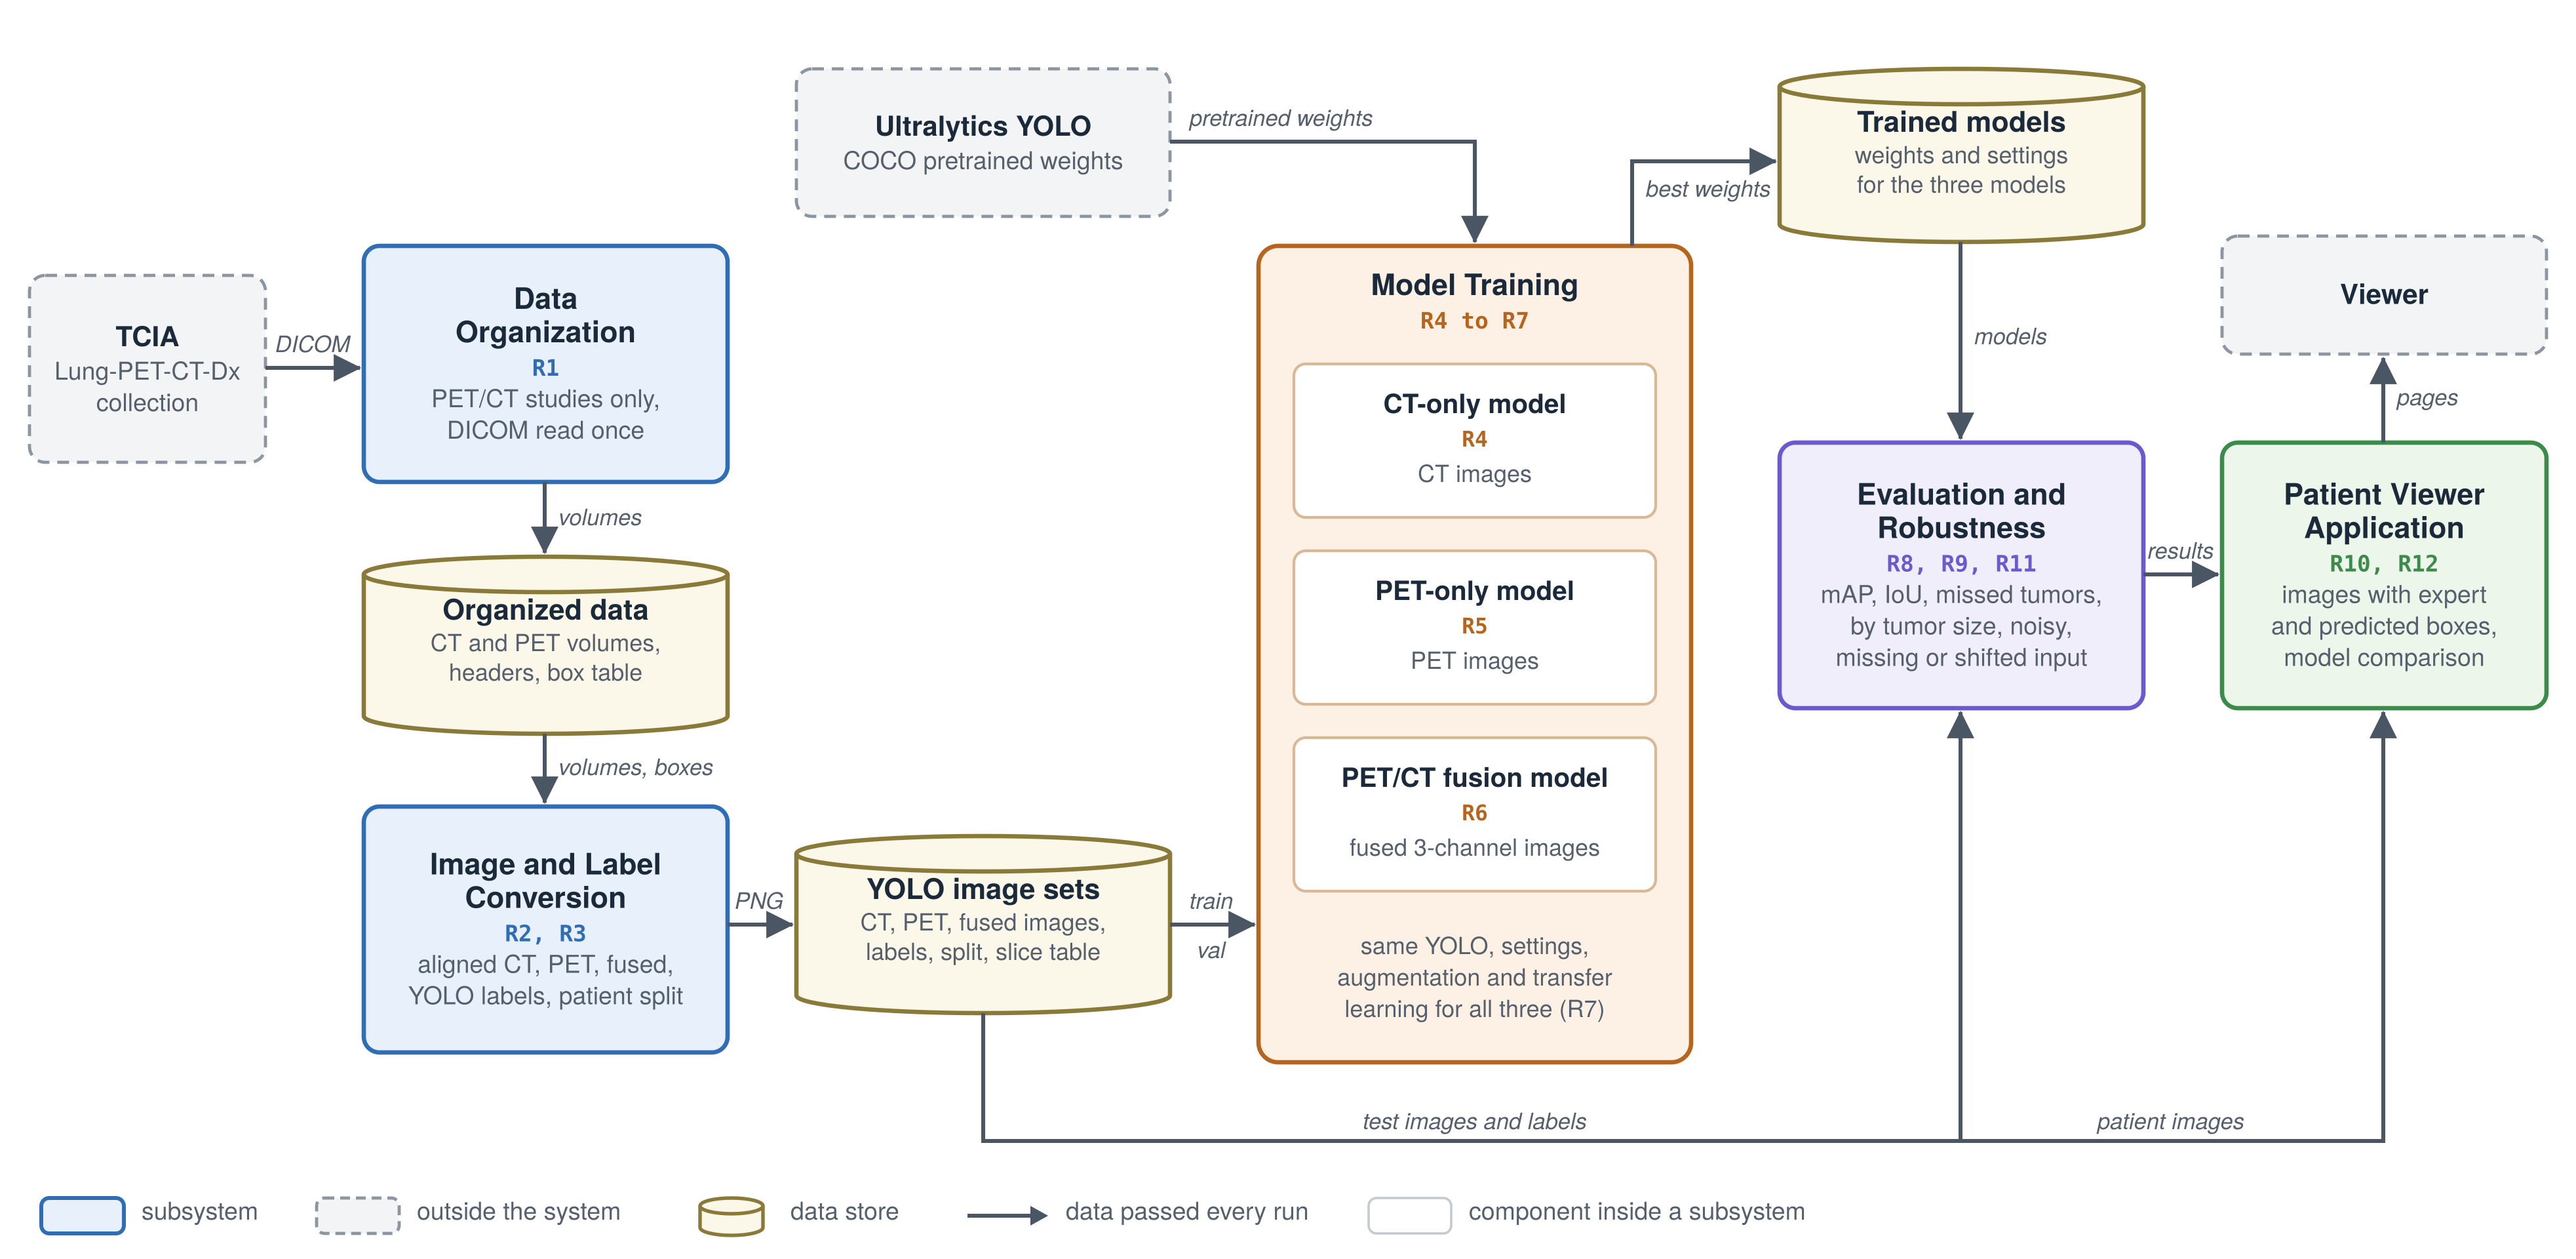
\includegraphics[width=\textwidth]{./figures/SA_P2_LungTumor.png}
	\caption[System architecture of the lung tumor detection system (drawn using Claude).]{\upd{System architecture of the lung tumor detection system (drawn using Claude).}}
	\label{fig:architecture}
\end{figure}

{\color{red}Figure~\ref{fig:architecture} presents the system architecture of ...

\noindent\textbf{Note from Dr.\ Sekmen.} Figure~\ref{fig:architecture} is the reference architecture for this project. Explain it here in your own words, starting with the sentence above. Walk the reader through the figure from left to right. For each subsystem, say what it is responsible for, what it receives, what it produces and which requirements of Chapter~2 it satisfies. Explain the three data stores, the outside sources (TCIA, the pretrained YOLO weights and the viewer) and what each arrow carries. Make clear that DICOM files are read only once, by Data Organization and Image and Label Conversion, and that everything after that works with PNG images and label files. Then add a short traceability table that lists every requirement R1 to R12 against the subsystem that satisfies it. Use the subsystem names of Figure~\ref{fig:architecture} everywhere in this chapter, and delete this red text when you are done.\par}

\upd{Data Organization} is a subsystem in our project that mainly focuses on the dataset we are using, as well as the organization of the dataset. Our project uses the dataset Lung-PET-CT-Dx collection from The Cancer Imaging Archive (TCIA)\upd{. It} contains two different series of scans, CT and PET\upd{. Only patients with a paired PET/CT study are kept, and studies} that do not contain annotations \upd{are excluded}. Each study is then checked for available expert tumor annotations\upd{.} The organized data and tumor annotations are then passed to \upd{Image and Label Conversion} for image preparation and image alignment.

The \upd{Image and Label Conversion} subsystem is responsible for preparing the collected images for tumor detection. Received CT images are processed using lung and mediastinal windows, while PET images are normalized and spatially aligned with the corresponding CT images. The received images are then put into three different input channels, CT-only, PET-only and \upd{PET/CT fusion}. The expert annotations are then converted into YOLO bounding box labels\upd{, and the patients are} split into three different sets, training, validation and testing\upd{, in proportions of} 75/10/15 respectively. The following images and labels are then passed into the next subsystem for model training \upd{and, for the test set, to evaluation. After this step the system no longer reads DICOM files.}

The \upd{Model Training} subsystem is where we apply training and deep learning models to detect tumors in the received images. A pretrained YOLO model is used to train the three independent tumor detection models. All three models will \upd{use} the same pretrained weights, patient data splits and training settings to keep the models on an even playing field for comparison. Once the models are trained and the test images are processed, the models will generate bounding boxes with confidence scores. With those confidence \upd{scores} they are able to be evaluated in the next subsystem\upd{, Evaluation and Robustness,} dealing with the comparison of those scores against each modality, specifically they are measured to compare tumor localization performance of each modality.

The \upd{Evaluation and Robustness} subsystem is responsible for analyzing the tumor detection results produced by the three YOLO models. The subsystem receives \upd{the trained models, runs them on the test images to obtain} predicted tumor bounding boxes and confidence scores\upd{,} and compares them against the expert-provided tumor annotations. The performance of the CT-only, PET-only, and fused PET/CT models is evaluated using metrics such as precision, recall, Intersection over Union (IoU), and mean Average Precision (mAP). Additional analysis examines tumor size, false positives, missed detections, and the effects of noisy, missing, or misaligned imaging data on model performance. \upd{The Patient Viewer Application} provides visual comparisons of the medical images, expert annotations, and predicted tumor locations through a reproducible application. These results allow the performance of the three imaging approaches to be compared and their strengths and limitations to be identified.

\upd{Figures~\ref{fig:team1} and \ref{fig:team2} show the inside of these subsystems in more detail.}

\begin{figure}[htbp]
	\centering
	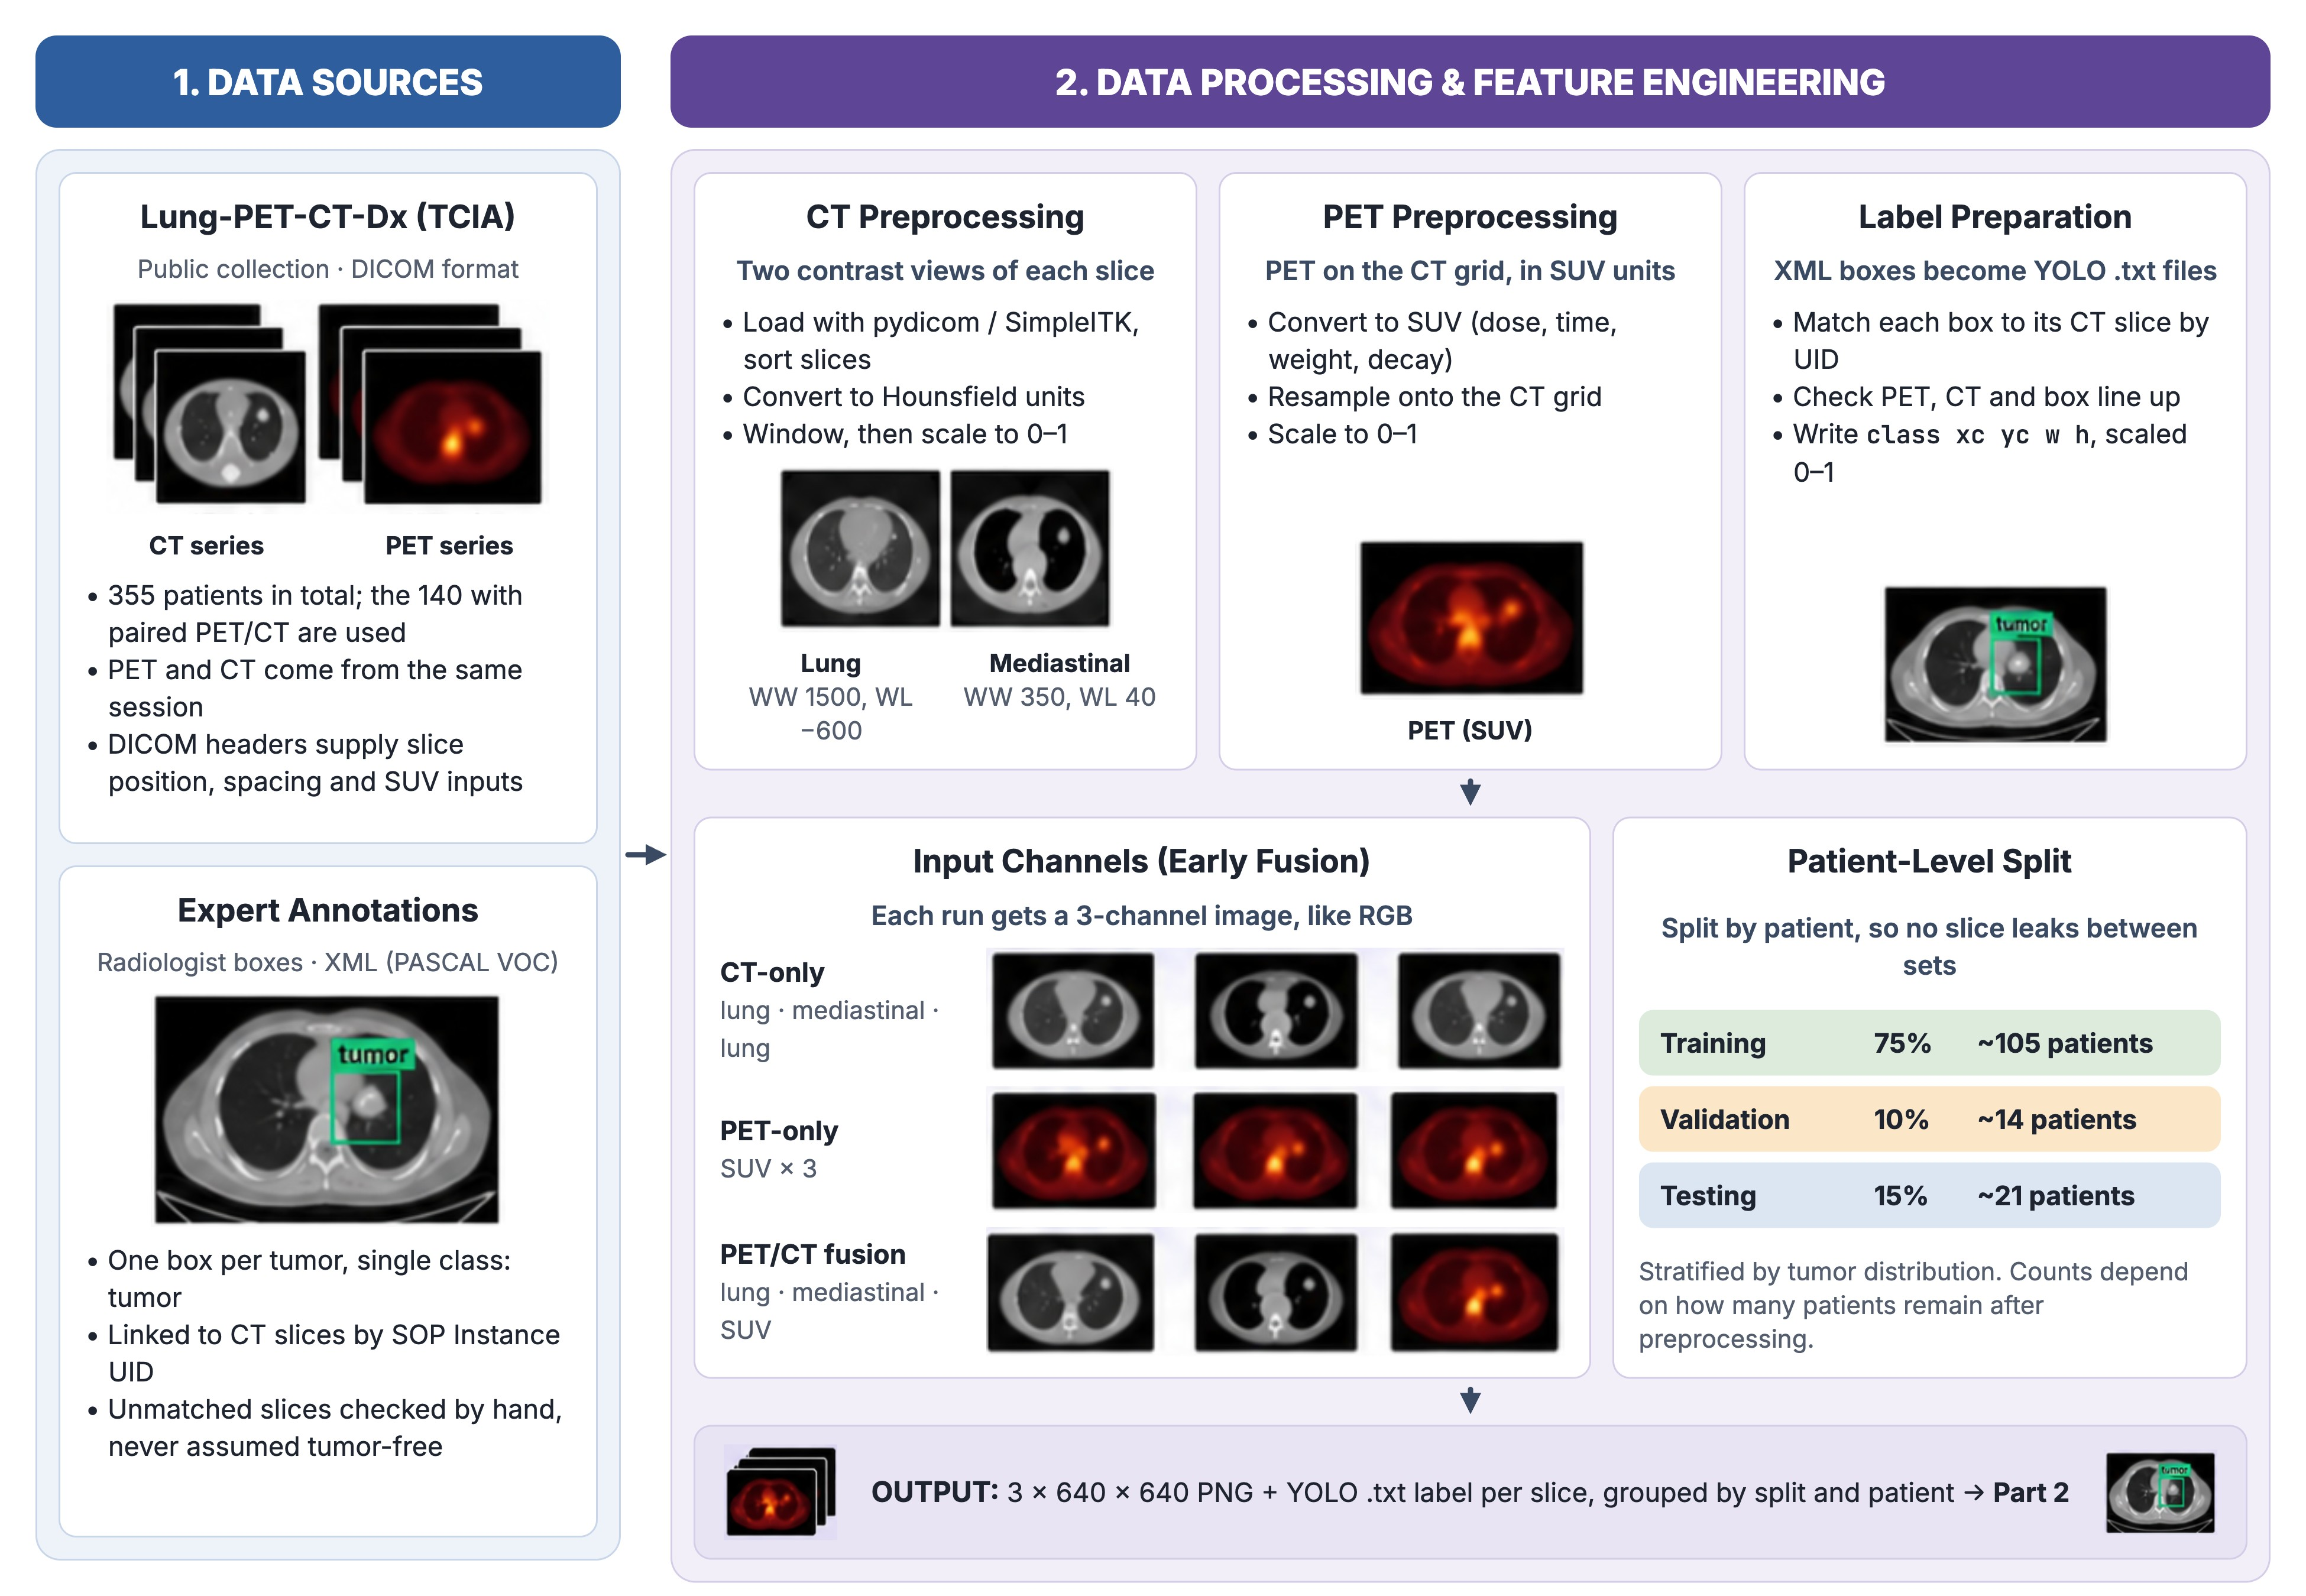
\includegraphics[width=\textwidth]{./figures/Team_DataSources_Processing.jpg}
	\caption[Data Organization and Image and Label Conversion.]{\upd{Data Organization and Image and Label Conversion.}}
	\label{fig:team1}
\end{figure}

\begin{figure}[htbp]
	\centering
	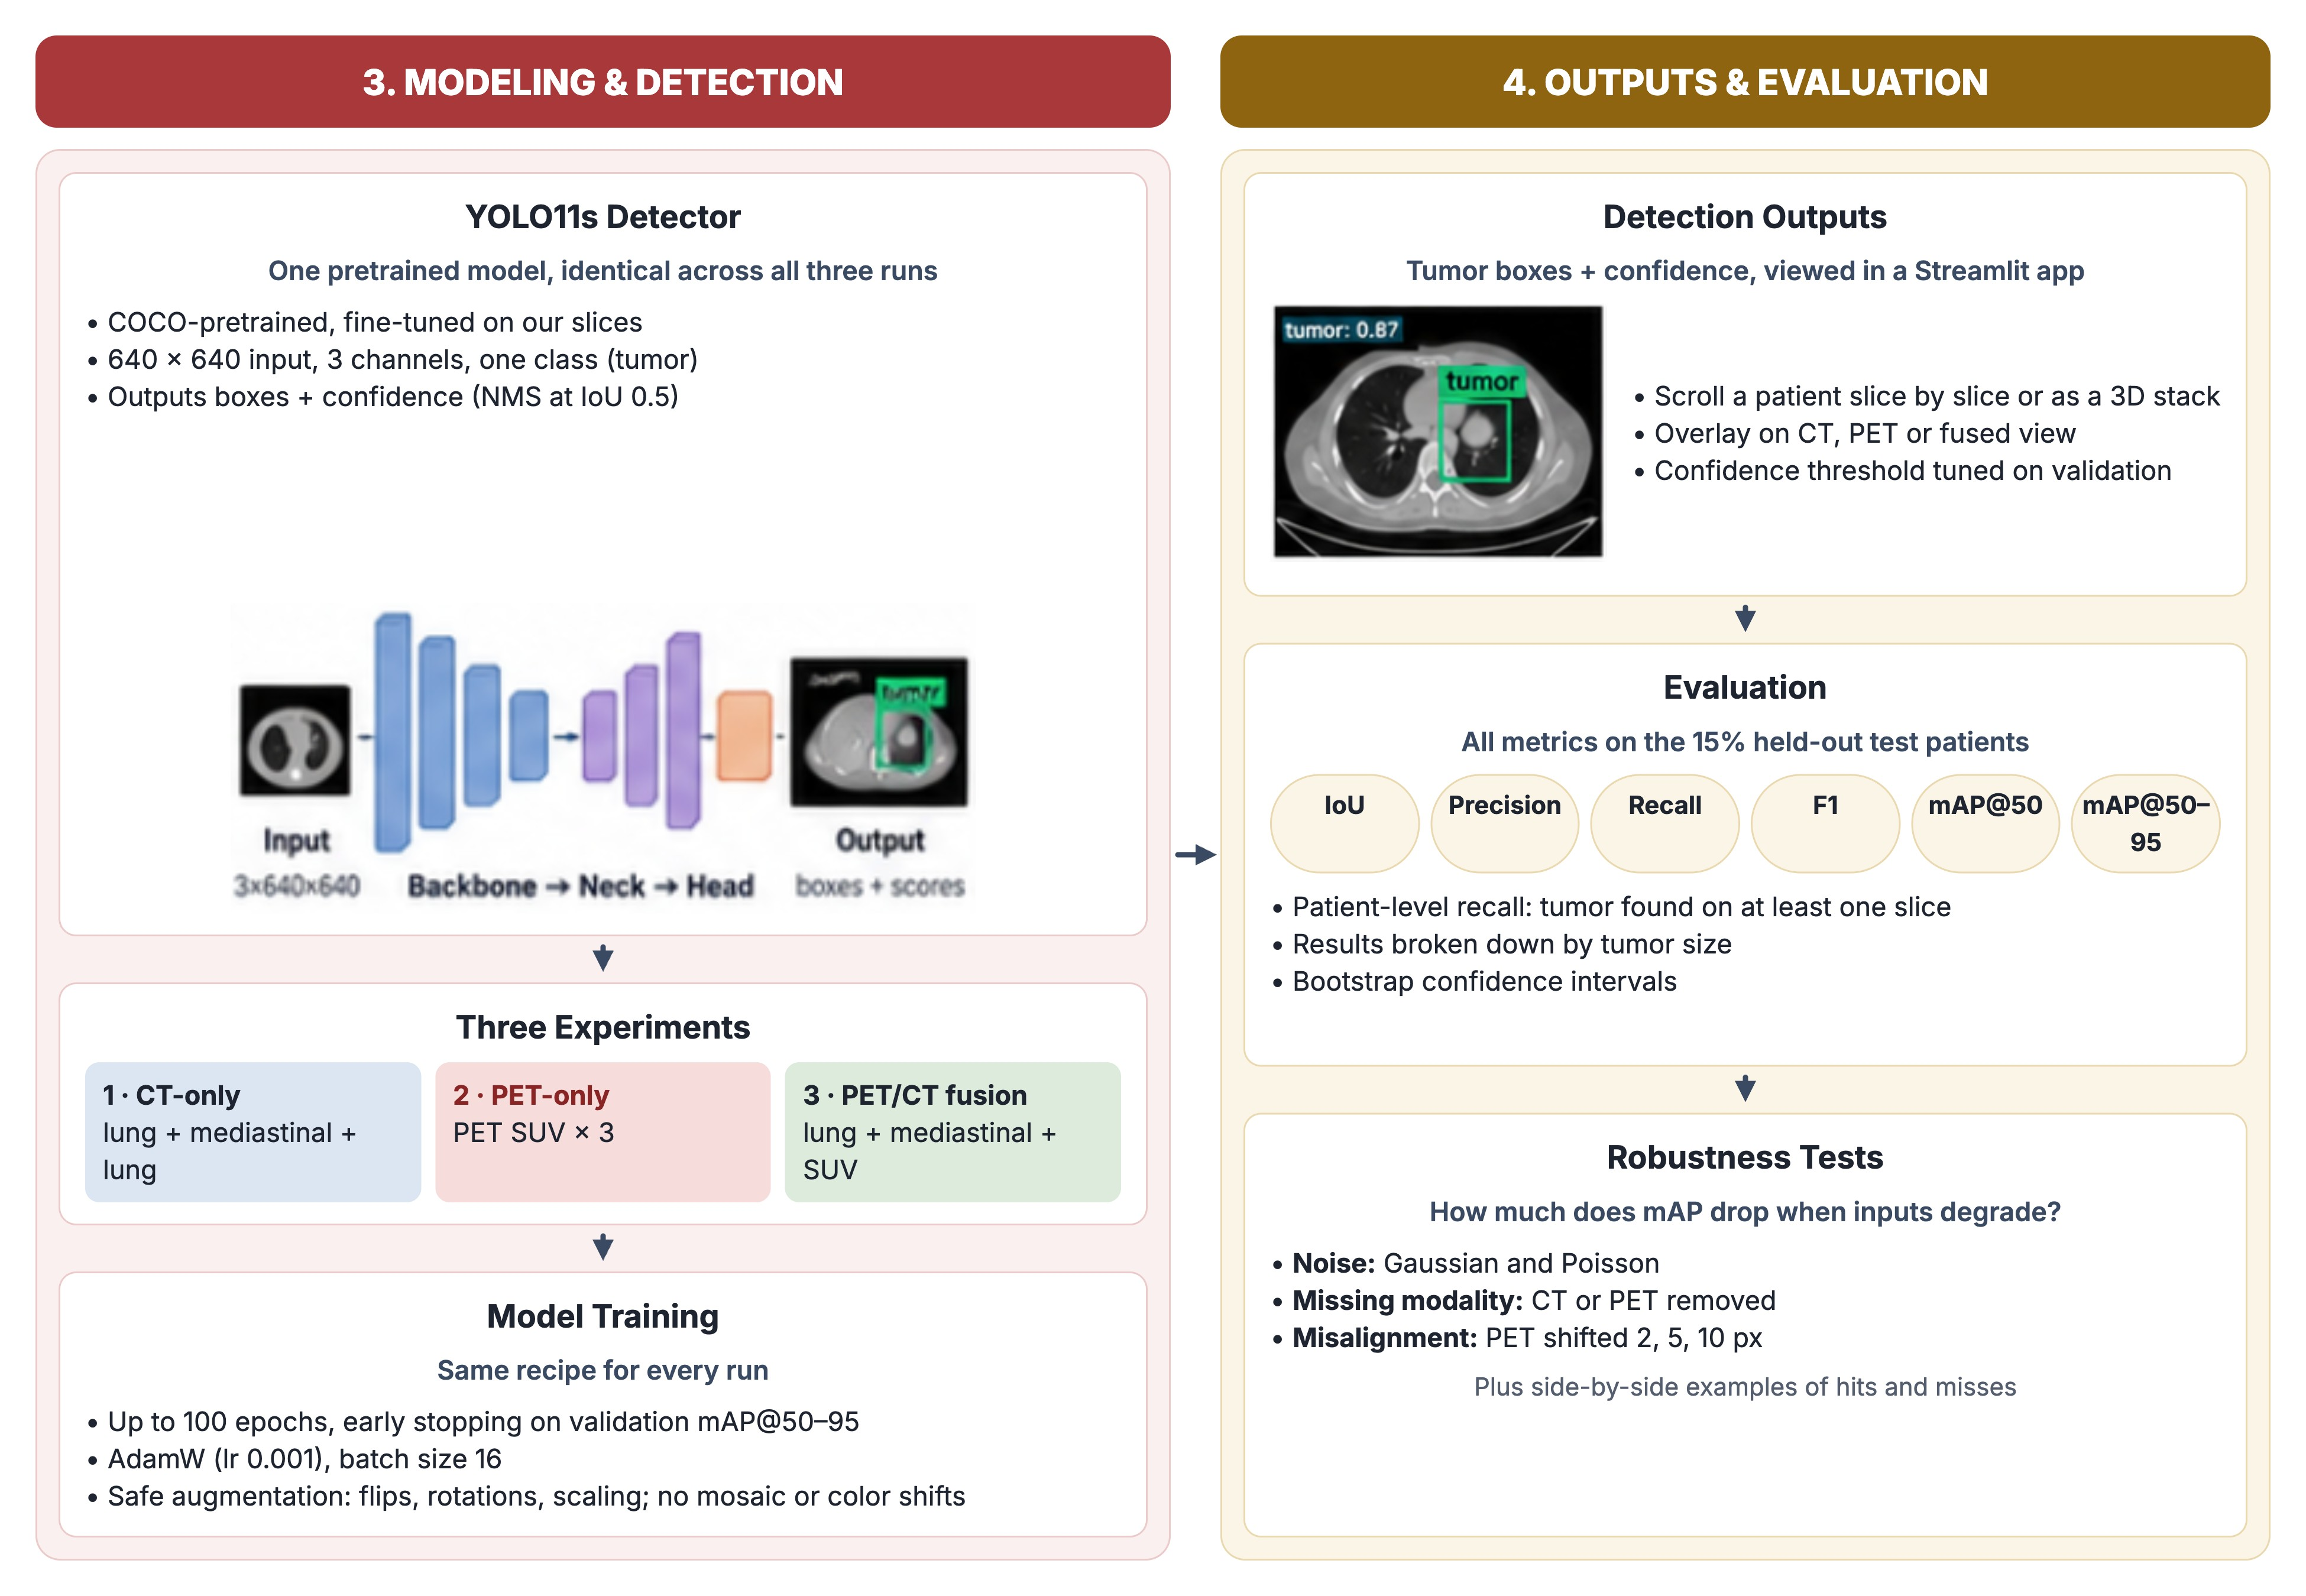
\includegraphics[width=\textwidth]{./figures/Team_Modeling_Outputs.jpg}
	\caption[Model Training, Evaluation and Robustness, and the Patient Viewer Application.]{\upd{Model Training, Evaluation and Robustness, and the Patient Viewer Application.}}
	\label{fig:team2}
\end{figure}

{\color{red}\noindent\textbf{Note from Dr.\ Sekmen.} Retitle the panels of Figures~\ref{fig:team1} and \ref{fig:team2} so they use the subsystem names of Figure~\ref{fig:architecture}. ``Data Sources'' becomes Data Organization, ``Data Processing \& Feature Engineering'' becomes Image and Label Conversion, ``Modeling \& Detection'' becomes Model Training, and ``Outputs \& Evaluation'' becomes Evaluation and Robustness together with the Patient Viewer Application.\par}

% ---------------------------------------------------------------------
\section{Detailed Design}
\label{sec:detailed}
This section explains how each of the \upd{subsystems in Figure~\ref{fig:architecture}} works inside. Each subsystem is divided into components (Figures~\upd{\ref{fig:comp-org} to \ref{fig:comp-eval}}), and the methods, formulas and settings of each component are given here.

% .....................................................................
\subsection[Data Organization]{\upd{Data Organization}}

\begin{figure}[htbp]
	\centering
	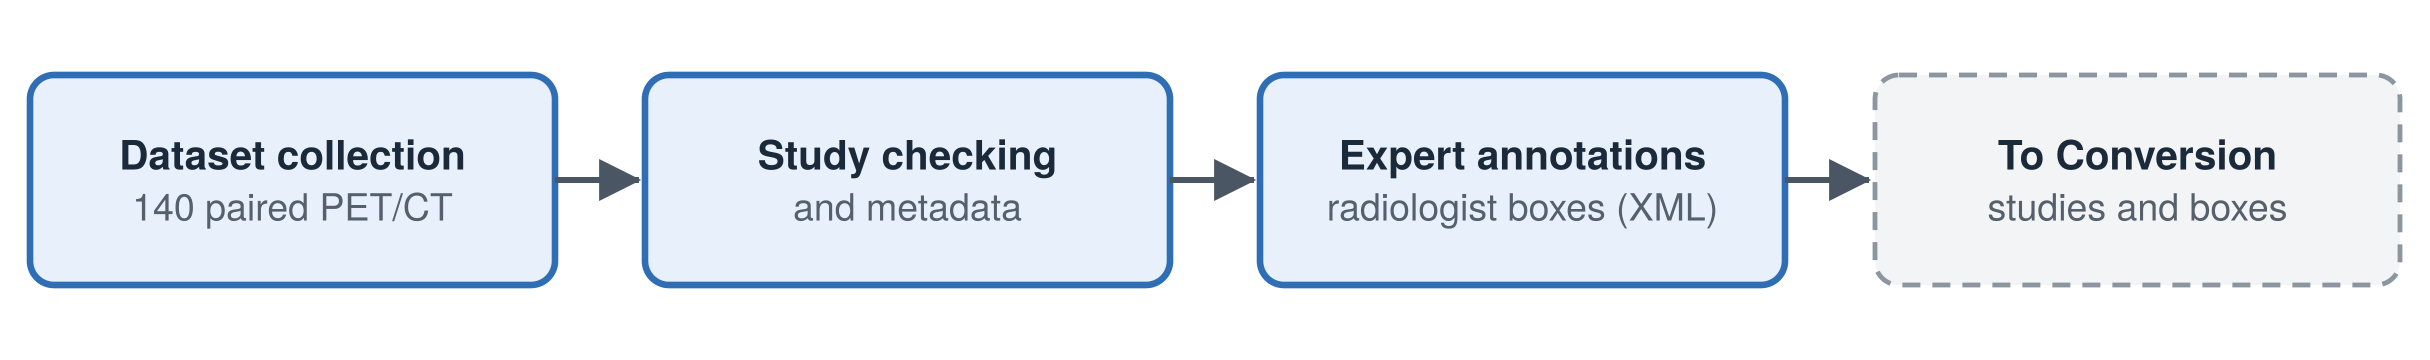
\includegraphics[width=\textwidth]{./figures/Comp_DataOrganization.png}
	\caption[Components of Data Organization.]{Components of \upd{Data Organization}.}
	\label{fig:comp-org}
\end{figure}

\textbf{Dataset collection.} The 140 patients with a paired PET/CT study are taken from the Lung-PET-CT-Dx collection, and the downloaded version is recorded for citation. The series of each patient are organized by patient identifier and passed to study checking.

\textbf{Study checking and metadata.} A study is kept only if its CT, PET and annotations are all present. The DICOM headers supply the slice position and pixel spacing, used for alignment and for tumor size in millimeters, and the dose, injection time, scan time and patient weight, used for the SUV conversion. Studies that cannot be matched reliably are documented and excluded, and the verified CT and PET volumes \upd{are stored in the organized data}.

\textbf{Expert annotations.} Each radiologist box (PASCAL VOC XML) marks one tumor on one CT slice and carries that slice's identifier, which links the box to its image. There is a single class, tumor. The verified boxes are \upd{stored with the volumes and passed to Image and Label Conversion}, where they are converted to YOLO labels.

% .....................................................................
\subsection[Image and Label Conversion]{\upd{Image and Label Conversion}}

\begin{figure}[htbp]
	\centering
	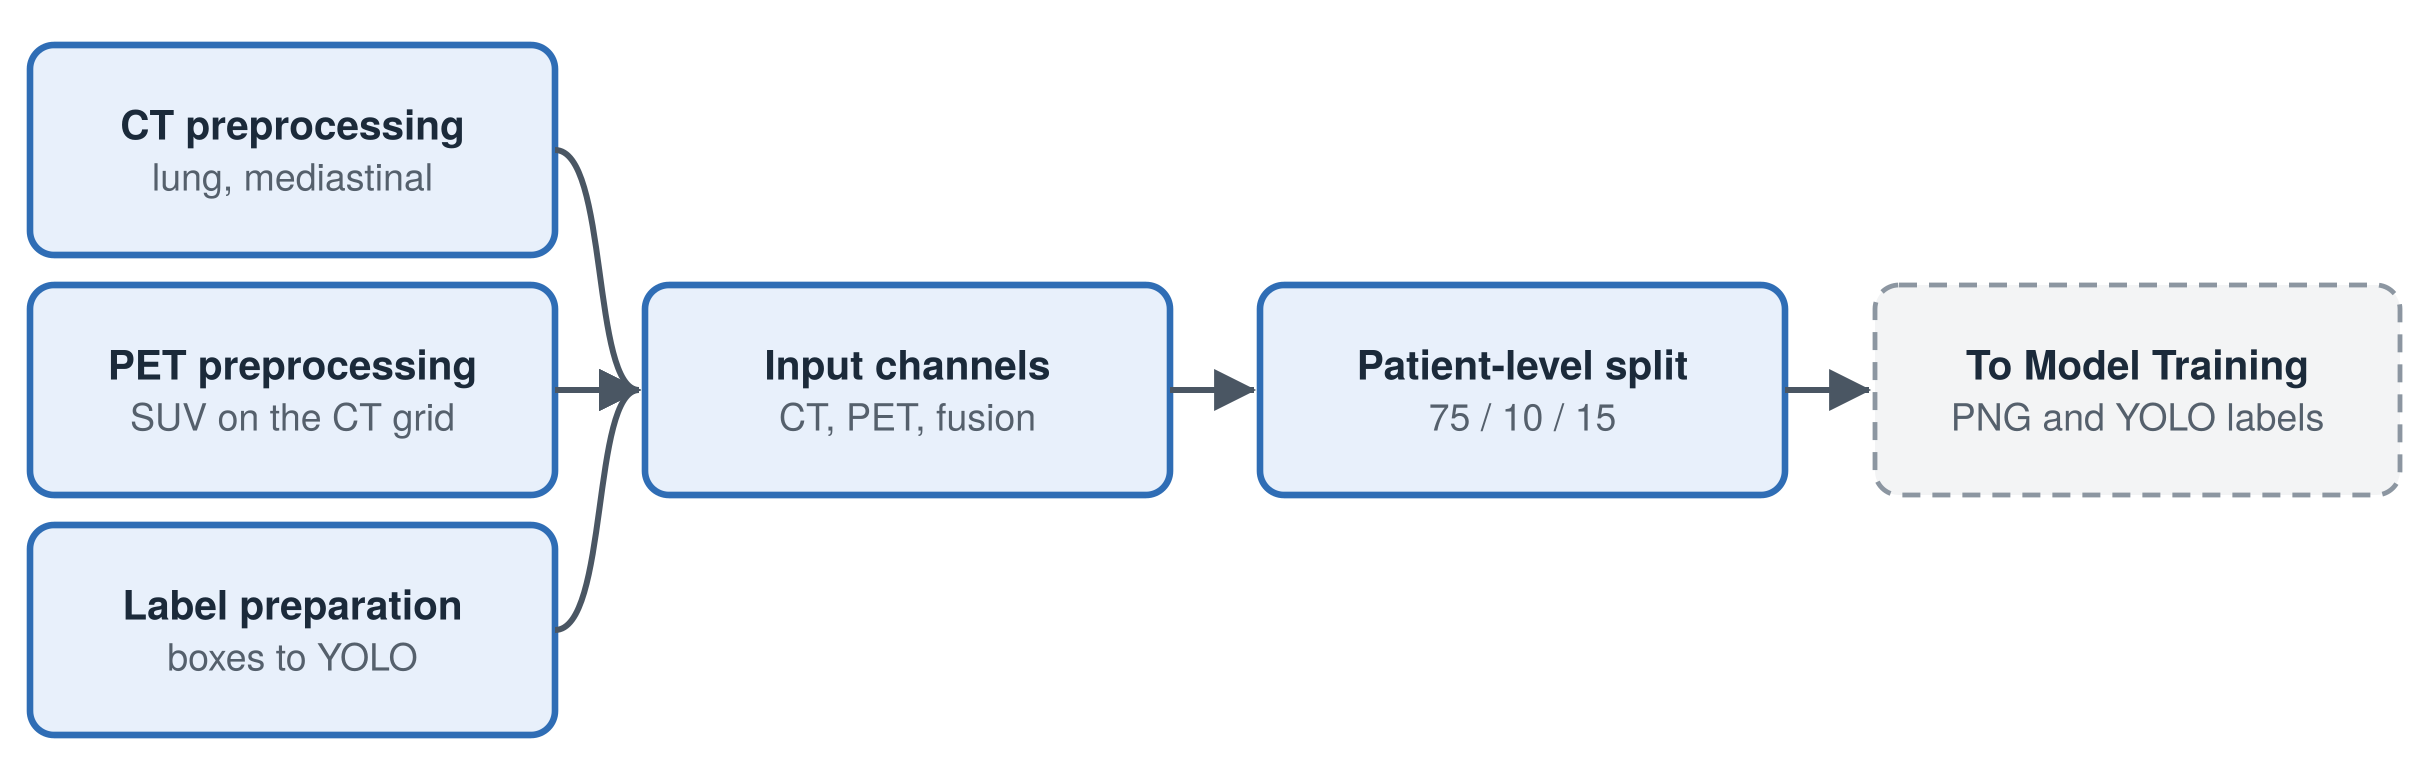
\includegraphics[width=\textwidth]{./figures/Comp_Conversion.png}
	\caption[Components of Image and Label Conversion.]{Components of \upd{Image and Label Conversion}.}
	\label{fig:comp-conv}
\end{figure}

\textbf{CT preprocessing.} CT slices are sorted by position and converted to Hounsfield units (HU). Each slice is windowed twice, with window width $WW$ and level $WL$, and scaled to 0--1:
\begin{equation}
	I = \mathrm{clip}\!\left(\frac{HU - (WL - WW/2)}{WW},\ 0,\ 1\right)
\end{equation}
The lung window ($WW = 1500$, $WL = -600$) covers $-1350$ to $150$ HU; the mediastinal window ($WW = 350$, $WL = 40$) covers $-135$ to $215$ HU. The two windowed images of each slice are passed to input channel construction.

\textbf{PET preprocessing.} Raw PET values are converted to standardized uptake values so they are comparable between patients:
\begin{equation}
	SUV = \frac{C \cdot W}{D_0 \cdot 2^{-\Delta t / T_{1/2}}}
\end{equation}
$C$ is the measured activity concentration, $W$ the patient weight, $D_0$ the injected dose, $\Delta t$ the time from injection to scan, and $T_{1/2}$ the tracer half-life (about 110 minutes for fluorine-18). The volume is then resampled onto the CT grid and scaled to 0--1 with a fixed upper limit of SUV 15. Values above 15 are clipped, so a value of 1 means the same uptake for every patient. The aligned PET images are passed to input channel construction.

\textbf{Label preparation.} Each box is matched to its CT slice by slice identifier (SOP Instance UID), checked against the PET and CT slices, and written as a YOLO line, with image width $W_{img}$ and height $H_{img}$:
\begin{equation}
	x_c = \frac{x_{min} + x_{max}}{2W_{img}}, \quad
	y_c = \frac{y_{min} + y_{max}}{2H_{img}}, \quad
	w = \frac{x_{max} - x_{min}}{W_{img}}, \quad
	h = \frac{y_{max} - y_{min}}{H_{img}}
\end{equation}
The values stay valid when images are resized to $640 \times 640$. Slices with no matching box are checked by hand and never assumed to be tumor-free. The labels stay linked to the CT, PET and fused images of the same slice\upd{, and the patient identifier and pixel spacing of every slice are recorded in a slice table, so later steps never need the DICOM files}.

\textbf{Input channel construction.} Each experiment gets a three-channel image (Table~\ref{tab:channels}). The fusion input stacks the CT lung window, the CT mediastinal window and the aligned PET SUV image, so the channels line up pixel by pixel. Using the same three-channel format for all experiments lets one pretrained detector be used unchanged. The images are saved as $640 \times 640$ PNG files and passed to the patient-level split.

\begin{table}[htbp]
	\centering
	\caption{Channel contents of the three experiments.}
	\label{tab:channels}
	\begin{tabular}{llll}
		\hline
		Experiment & Channel 1 & Channel 2 & Channel 3 \\
		\hline
		CT-only & CT lung window & CT mediastinal window & CT lung window \\
		PET-only & PET SUV & PET SUV & PET SUV \\
		PET/CT fusion & CT lung window & CT mediastinal window & PET SUV \\
		\hline
	\end{tabular}
\end{table}

\textbf{Patient-level split.} Whole patients are assigned to training, validation and testing (about 105, 14 and 21 of 140), stratified by tumor distribution. Splitting by patient keeps near-identical neighboring slices out of different sets, and a check confirms no patient appears in more than one set. The same split is used for all three experiments. The image folders, YOLO label files\upd{, slice table} and dataset configuration files are then \upd{stored in the YOLO image sets}.

% .....................................................................
\subsection[Model Training]{\upd{Model Training}}

\begin{figure}[htbp]
	\centering
	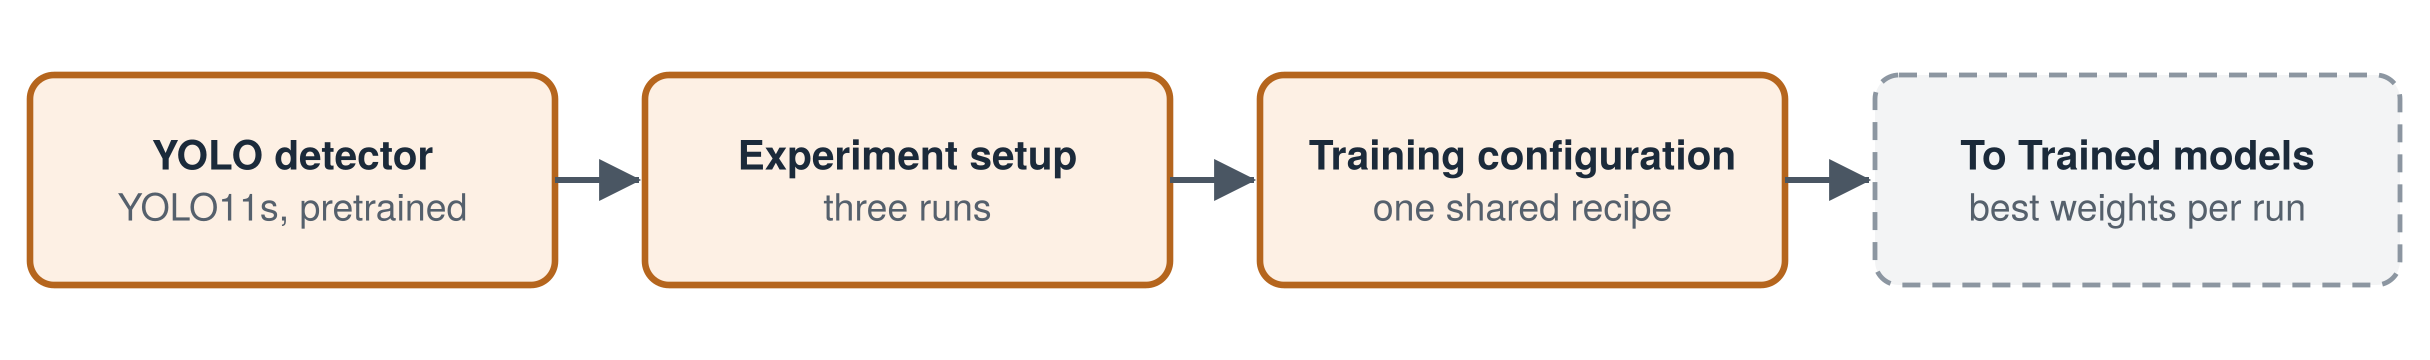
\includegraphics[width=\textwidth]{./figures/Comp_ModelTraining.png}
	\caption[Components of Model Training.]{Components of \upd{Model Training}.}
	\label{fig:comp-train}
\end{figure}

\textbf{YOLO detector.} The detector is YOLO11s, fine-tuned from COCO-pretrained weights. It takes a $640 \times 640$, three-channel image: a backbone extracts features, a neck combines several scales so small and large tumors are both found, and a head predicts boxes and confidence scores for one class, tumor. The same architecture is used for all three experiments.

\textbf{Experiment setup.} The CT-only, PET-only and fusion detectors are trained as three independent runs, each with its own dataset file but with the same starting weights, split and recipe, so only the image content differs. No weights are carried from one experiment to another.

\textbf{Training configuration.} The recipe in Table~\ref{tab:recipe} is applied to every run, and the weights from the best validation epoch are kept. Mosaic and color changes are off because they would mix slices from different patients or mix the CT and PET channels. The configuration and the trained weights are saved separately for each experiment \upd{in the trained models store}.

\begin{table}[htbp]
	\centering
	\caption{Training recipe shared by all three experiments.}
	\label{tab:recipe}
	\begin{tabular}{lp{10cm}}
		\hline
		Input & $640 \times 640$, 3 channels, one class (tumor) \\
		Epochs & Up to 100; early stopping on validation mAP@50--95 (patience 20 epochs) \\
		Optimizer & AdamW, learning rate 0.001, batch size 16 \\
		Augmentation & Flips, rotations, scaling; training images only; no mosaic, no color changes \\
		Random seed & Fixed at 0 and the same for all runs \\
		\hline
	\end{tabular}
\end{table}

% .....................................................................
\subsection[Evaluation and Robustness]{\upd{Evaluation and Robustness}}

\begin{figure}[htbp]
	\centering
	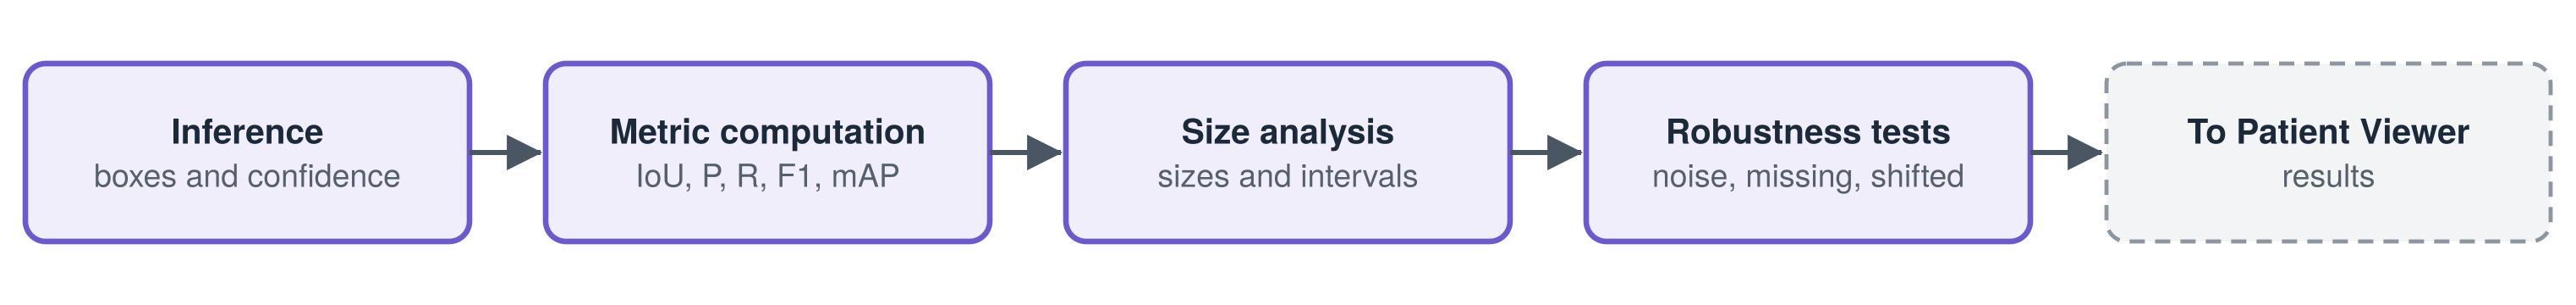
\includegraphics[width=\textwidth]{./figures/Comp_Evaluation.png}
	\caption[Components of Evaluation and Robustness.]{Components of \upd{Evaluation and Robustness}.}
	\label{fig:comp-eval}
\end{figure}

\textbf{Inference.} Each model runs on the test images of its own experiment, and overlapping boxes for the same tumor are merged by non-maximum suppression at an IoU of 0.5. The confidence threshold is chosen on the validation set and then fixed for testing. Each prediction is saved with its patient and slice identifier\upd{.}

\textbf{Metric computation.} A predicted box $P$ is matched to an expert box $E$ by Intersection over Union:
\begin{equation}
	IoU = \frac{\mathrm{area}(P \cap E)}{\mathrm{area}(P \cup E)}
\end{equation}
A match at $IoU \geq 0.5$ (the same value used for non-maximum suppression and for mAP@50) is a true positive ($TP$), an unmatched prediction is a false positive ($FP$), and an unmatched expert box is a false negative ($FN$). The same rule is used for all three models.
\begin{equation}
	\mathrm{Precision} = \frac{TP}{TP + FP}, \quad
	\mathrm{Recall} = \frac{TP}{TP + FN}, \quad
	F_1 = \frac{2 \cdot \mathrm{Precision} \cdot \mathrm{Recall}}{\mathrm{Precision} + \mathrm{Recall}}
\end{equation}
mAP@50 is the mean average precision at IoU 0.5, and mAP@50--95 averages it over IoU 0.50 to 0.95 in steps of 0.05. A patient-level recall counts a tumor as found if at least one of its slices has a matching detection. The results of all three models are saved in one common format so they can be compared directly.

\textbf{Size analysis and intervals.} Tumor size is calculated in millimeters from each expert box and the \upd{pixel spacing in the slice table}, and each tumor is placed in one group by the longer side of its box: small (under 20 mm), medium (20 to 40 mm) or large (over 40 mm). The limits are fixed before the analysis and saved with the evaluation settings. Because only about 21 patients are tested, the test patients are resampled with replacement 1,000 times, every metric is recomputed, and the middle 95\% of values is reported as the interval. The component also compares the saved predictions case by case, to find tumors that one model detects and another misses, and to list the false positives and missed tumors of each model, including cases where the fused model differs from CT-only or PET-only.

\textbf{Robustness tests.} Degradations are applied to copies of the test images and the trained models are not retrained. Gaussian and Poisson noise are applied to all three models. For the fusion model, either the CT channels or the PET channel is removed, and the PET channel is shifted by 2, 5 or 10 pixels. The drop is measured against the clean result:
\begin{equation}
	\Delta mAP = mAP_{clean} - mAP_{degraded}
\end{equation}
The results are saved for each model and test condition, which shows how sensitive the three approaches are to noise, missing information and misalignment.

% .....................................................................
\subsection[Patient Viewer Application]{\upd{Patient Viewer Application}}

\textbf{Detection viewer.} A Streamlit application lets a reviewer pick a test patient, scroll the slices or step through the 3D stack, and view predicted boxes with confidence scores on the CT, PET or fused view. It only reads saved images and predictions, so it shows exactly what was evaluated. The final results, representative images and robustness comparisons are available through the \upd{same} application.

\end{document}
